% The BOBILib paper, in the format of SPIE proceedings (spie.cls from TeX Live's
% texlive-publishers). Build from bobilib/paper:  make paper  (latexmk -pdf main.tex,
% pdflatex + bibtex). Needs generated/facts.tex (make data), figures/*.pdf (make figures),
% refs.bib and spiebib-doi.bst. Every computed result quoted in the text, the tables and the
% captions is a macro of generated/facts.tex, computed from bobilib/results/. Typed numbers are
% instance parameters (sizes, densities, budgets), settings (tolerances, time limits, software
% versions), the settings of published runs, and the toy numbers of the explainer figures.
\documentclass[]{spie}  % US letter, 10 pt, Times

% Placeholders for the author to fill in.
\newcommand{\authoremail}{EMAIL}
\newcommand{\repourl}{REPOSITORY-URL}
\newcommand{\datadoi}{DATA-DOI}

\usepackage[T1]{fontenc}
\usepackage{mathptmx}
\renewcommand{\ttdefault}{lmtt}
\usepackage{authblk}
\usepackage{amsmath,amssymb}
\let\proof\relax\let\endproof\relax  % spie.cls defines \proof, amsthm defines it again
\usepackage{amsthm}
\usepackage{graphicx}
\usepackage{array,booktabs}
\usepackage{siunitx}
\usepackage{capt-of}
\usepackage{needspace}
\usepackage{xurl}
\urlstyle{same}
\usepackage[hidelinks]{hyperref}

% Generated by paper/scripts/gen_facts.py from bobilib/results/; do not edit by hand.
% Each macro is computed from the results files and checked against the paper spec.
% Integers use {,} as thousands separator; percentages are bare numbers (add \%).

\newcommand{\NumInstances}{2{,}654}% BOBILib instances
\newcommand{\NumBobiOptimal}{1{,}027}% BOBILib status optimal
\newcommand{\NumBobiInfeasible}{33}% BOBILib status infeasible
\newcommand{\NumBobiFeasible}{1{,}175}% BOBILib status feasible
\newcommand{\NumBobiOpen}{419}% BOBILib status open
\newcommand{\NumUnsolved}{1{,}594}% feasible or open in BOBILib
\newcommand{\NumLitOptimal}{527}% already optimal in published work
\newcommand{\NumNewOptimal}{81}% proven optimal here
\newcommand{\NumNoFeasible}{40}% no bilevel feasible point (here)
\newcommand{\NumFirstPoint}{230}% first verified point here, BOBILib has none
\newcommand{\NumUnchanged}{716}% status unchanged
\newcommand{\NumSettled}{648}% settled = literature + new optimal + no feasible point
\newcommand{\PctSettled}{41}% settled share of the unsolved, percent
\newcommand{\NumOptimalNow}{608}% optimal now among the unsolved
\newcommand{\NumPacking}{1{,}254}% packing interdiction among the unsolved
\newcommand{\PctPacking}{79}% packing share of the unsolved, percent
\newcommand{\NumKipUnsolved}{392}% KIP not optimal in BOBILib
\newcommand{\NumMkipUnsolved}{862}% MKIP not optimal in BOBILib
\newcommand{\NumCliqueUnsolved}{60}% clique not optimal in BOBILib
\newcommand{\NumNetworkUnsolved}{2}% network not optimal in BOBILib
\newcommand{\NumGeneralizedUnsolved}{12}% generalized not optimal
\newcommand{\NumGeneralPure}{131}% general pure not optimal (incl. infeasible)
\newcommand{\NumGeneralMixed}{168}% general mixed not optimal (incl. infeasible)
\newcommand{\NumGeneralUnsolved}{266}% general feasible or open (not infeasible)
\newcommand{\NumKipInstances}{599}% BOBILib knapsack instances
\newcommand{\NumMkipInstances}{954}% BOBILib multidim-knapsack instances
\newcommand{\NumCliqueInstances}{220}% BOBILib clique instances
\newcommand{\NumNetworkInstances}{72}% BOBILib network instances
\newcommand{\NumGeneralizedInstances}{90}% BOBILib generalized instances
\newcommand{\NumAssignmentInstances}{24}% BOBILib assignment instances
\newcommand{\NumGeneralInstances}{695}% BOBILib general (MIPLIB-derived and other) instances
\newcommand{\NumLitKip}{376}% KIP optima of Weninger and Fukasawa
\newcommand{\NumLitLozano}{96}% optima of Lozano, Bergman and Cire (all families)
\newcommand{\NumLitOr}{87}% OR optima of Lozano et al.
\newcommand{\NumLitGeneralized}{4}% generalized optima of Lozano et al.
\newcommand{\NumLitMiplibLozano}{5}% MIPLIB 3 optima of Lozano et al.
\newcommand{\NumLitImkp}{52}% imkp optima of Fischetti et al. 2019
\newcommand{\NumLitMkip}{139}% MKIP literature optima (OR + imkp)
\newcommand{\NumLitMiplib}{8}% MIPLIB-derived literature optima
\newcommand{\NumLitFischettiSeventeen}{1}% air03-0.100000
\newcommand{\NumLitVasquez}{1}% p0282-0.500000
\newcommand{\NumLitEarlierRelease}{1}% neos-950242_0_100
\newcommand{\NumKipFiles}{583}% KIP files at published optima
\newcommand{\NumKipBobiAbove}{335}% KIP with BOBILib value above the published optimum
\newcommand{\KipBobiExcessMedian}{8}% median excess, percent
\newcommand{\KipBobiExcessMax}{672}% largest excess, percent
\newcommand{\ImkpBobiExcessMax}{23}% largest imkp excess over the optimum, percent
\newcommand{\NumNewKip}{16}% KIP optima proven here
\newcommand{\NumNewClique}{57}% clique optima proven here
\newcommand{\NumNewNetwork}{2}% network optima proven here
\newcommand{\NumNewHpr}{5}% MIPLIB-bound optima
\newcommand{\NumNewOr}{1}% OR closure
\newcommand{\NumRayExact}{38}% rays checked in exact arithmetic
\newcommand{\NumRayFloat}{2}% rays checked in floating point only
\newcommand{\NumOrFirstAnywhere}{88}% OR first points anywhere
\newcommand{\NumOrPointNewToBobilib}{52}% OR points where the literature had one, BOBILib none
\newcommand{\NumOrFirstPoints}{140}% OR points where BOBILib has none
\newcommand{\NumGeneralPoints}{62}% general first points without coupling
\newcommand{\NumCoupledPoints}{28}% general first points with coupling
\newcommand{\NumGeneralFirstPoints}{90}% general first points
\newcommand{\NumMkipUnchanged}{582}% MKIP unchanged
\newcommand{\NumCliqueOpen}{3}% clique still open
\newcommand{\NumGeneralizedUnchanged}{8}% generalized unchanged
\newcommand{\NumGeneralUnchanged}{123}% general unchanged
\newcommand{\NumGeneralNew}{135}% general instances settled or given a first point here
\newcommand{\KipOpenItemsMin}{200}% fewest items among the 16
\newcommand{\KipOpenItemsMax}{500}% most items among the 16
\newcommand{\NumKipSubsetSum}{8}% class 6 (subset sum)
\newcommand{\NumKipEvenOdd}{8}% class 7 (even-odd)
\newcommand{\NumKipOptEqualsBobi}{16}% optimum = BOBILib value
\newcommand{\KipHardestName}{interKP-500-100-6-3}% slowest of the 16 (CPU)
\newcommand{\KipHardestOptimum}{6{,}976}% its optimum
\newcommand{\KipHardestNodes}{10{,}079}% its search nodes
\newcommand{\KipHardestCpu}{10.0}% its CPU seconds (one thread)
\newcommand{\KipHardestIndepNodes}{10{,}116}% nodes of scripts/ss_check.py on it
\newcommand{\KipMostNodesName}{interKP-300-100-6-3}% instance with the most nodes
\newcommand{\KipMostNodes}{19{,}405}% most nodes among the 16
\newcommand{\KipTotalCpu}{32.5}% CPU seconds for all 16
\newcommand{\NumKipEasy}{12}% the 16 other than class 6, budget index 3
\newcommand{\KipEasyMaxCpu}{0.26}% slowest of those 12, CPU s
\newcommand{\KipEasyMaxNodes}{651}% most nodes among those 12
\newcommand{\KipMedianNodes}{334.5}% median nodes of the 16
\newcommand{\KipMedianCpu}{0.155}% median CPU s of the 16
\newcommand{\NumKipPrevSolved}{12}% instances the previous search version proved
\newcommand{\KipPrevMaxSeconds}{427}% slowest proof of the previous version, s
\newcommand{\NumOr}{810}% OR instances
\newcommand{\NumOrPoints}{690}% verified OR points
\newcommand{\NumOrBetter}{469}% points strictly better than every published value
\newcommand{\NumOrNoPublished}{139}% OR instances without a published point
\newcommand{\NumOrBetterLb}{191}% better lower bounds (all variant -100)
\newcommand{\NumOrBetterLbNotOne}{0}% better lower bounds outside -100
\newcommand{\NumOrOneKnapsack}{270}% one follower knapsack (-100)
\newcommand{\NumOrOneKnapsackPoints}{270}% points there
\newcommand{\NumOrSeveral}{540}% several follower knapsacks (-0, -50)
\newcommand{\NumOrSeveralPoints}{420}% points there
\newcommand{\NumOrSeveralHigh}{360}% several knapsacks, budget 50% or 75%
\newcommand{\NumOrSeveralHighPoints}{360}% all certified
\newcommand{\NumOrSeveralQuarter}{180}% several knapsacks, budget 25%
\newcommand{\NumOrSeveralQuarterPoints}{60}% certified at 25%
\newcommand{\NumOrSeveralQuarterNoPoint}{120}% without a point at 25%
\newcommand{\OrGapOneQuarterLit}{24.0}% median published gap, variant -100, budget 0.25
\newcommand{\OrGapOneQuarterNow}{4.1}% median gap now, variant -100, budget 0.25
\newcommand{\OrPairedOneQuarter}{90}% instances in that median
\newcommand{\OrGapOneHalfLit}{34.0}% median published gap, variant -100, budget 0.50
\newcommand{\OrGapOneHalfNow}{7.1}% median gap now, variant -100, budget 0.50
\newcommand{\OrPairedOneHalf}{90}% instances in that median
\newcommand{\OrGapOneThreeQuarterLit}{0.14}% median published gap, variant -100, budget 0.75
\newcommand{\OrGapOneThreeQuarterNow}{0.14}% median gap now, variant -100, budget 0.75
\newcommand{\OrPairedOneThreeQuarter}{90}% instances in that median
\newcommand{\OrGapZeroQuarterLit}{33.3}% median published gap, variant -0, budget 0.25
\newcommand{\OrGapZeroQuarterNow}{31.4}% median gap now, variant -0, budget 0.25
\newcommand{\OrPairedZeroQuarter}{55}% instances in that median
\newcommand{\OrNoPointZeroQuarter}{31}% no published point, -0, 0.25
\newcommand{\OrFirstZeroQuarter}{0}% first points among those
\newcommand{\OrGapZeroHalfLit}{36.6}% median published gap, variant -0, budget 0.50
\newcommand{\OrGapZeroHalfNow}{29.1}% median gap now, variant -0, budget 0.50
\newcommand{\OrPairedZeroHalf}{59}% instances in that median
\newcommand{\OrNoPointZeroHalf}{31}% no published point, -0, 0.50
\newcommand{\OrFirstZeroHalf}{31}% first points among those
\newcommand{\OrGapZeroThreeQuarterLit}{5.1}% median published gap, variant -0, budget 0.75
\newcommand{\OrGapZeroThreeQuarterNow}{0.04}% median gap now, variant -0, budget 0.75
\newcommand{\OrPairedZeroThreeQuarter}{63}% instances in that median
\newcommand{\OrNoPointZeroThreeQuarter}{27}% no published point, -0, 0.75
\newcommand{\OrFirstZeroThreeQuarter}{27}% first points among those
\newcommand{\OrGapFiftyQuarterLit}{29.6}% median published gap, variant -50, budget 0.25
\newcommand{\OrGapFiftyQuarterNow}{28.2}% median gap now, variant -50, budget 0.25
\newcommand{\OrPairedFiftyQuarter}{70}% instances in that median
\newcommand{\OrNoPointFiftyQuarter}{20}% no published point, -50, 0.25
\newcommand{\OrFirstFiftyQuarter}{0}% first points among those
\newcommand{\OrGapFiftyHalfLit}{41.3}% median published gap, variant -50, budget 0.50
\newcommand{\OrGapFiftyHalfNow}{34.8}% median gap now, variant -50, budget 0.50
\newcommand{\OrPairedFiftyHalf}{70}% instances in that median
\newcommand{\OrNoPointFiftyHalf}{20}% no published point, -50, 0.50
\newcommand{\OrFirstFiftyHalf}{20}% first points among those
\newcommand{\OrGapFiftyThreeQuarterLit}{11.8}% median published gap, variant -50, budget 0.75
\newcommand{\OrGapFiftyThreeQuarterNow}{1.4}% median gap now, variant -50, budget 0.75
\newcommand{\OrPairedFiftyThreeQuarter}{80}% instances in that median
\newcommand{\OrNoPointFiftyThreeQuarter}{10}% no published point, -50, 0.75
\newcommand{\OrFirstFiftyThreeQuarter}{10}% first points among those
\newcommand{\OrClosureName}{OR10x100-0.75\_4.dat-0}% the OR instance closed here
\newcommand{\OrClosureValue}{8{,}813}% its optimum
\newcommand{\OrClosureLitLb}{8{,}814}% published (inconsistent) lower bound
\newcommand{\NumOrInconsistent}{4}% OR instances whose published lower bound exceeds the published point
\newcommand{\NumOrLitOptimalPoint}{69}% published OR optima reproduced by a file here
\newcommand{\NumCliqueSet}{60}% instances of the clique set
\newcommand{\NumCliqueSevenThree}{27}% density 0.7 with value 3
\newcommand{\NumCliqueNineFour}{30}% density 0.9 with value 4
\newcommand{\CliqueBobiMin}{5}% smallest BOBILib value
\newcommand{\CliqueBobiMax}{13}% largest BOBILib value
\newcommand{\CliqueMantelLhsForty}{410}% m-k at n=40, d=0.7
\newcommand{\CliqueMantelRhsForty}{400}% floor(n^2/4) at n=40
\newcommand{\CliqueBrouwerLhsForty}{527}% m-k at n=40, d=0.9
\newcommand{\CliqueBrouwerRhsForty}{522}% t_3(n)-floor(n/3)+2 at n=40
\newcommand{\CliqueTuranForty}{533}% t_3(n) at n=40
\newcommand{\CliqueKFortySeven}{136}% budget k at n=40, d=0.7
\newcommand{\CliqueMFortySeven}{546}% edges m at n=40, d=0.7
\newcommand{\CliqueKFortyNine}{175}% budget k at n=40, d=0.9
\newcommand{\CliqueMFortyNine}{702}% edges m at n=40, d=0.9
\newcommand{\CliqueMantelLhsFifty}{643}% m-k at n=50, d=0.7
\newcommand{\CliqueMantelRhsFifty}{625}% floor(n^2/4) at n=50
\newcommand{\CliqueBrouwerLhsFifty}{827}% m-k at n=50, d=0.9
\newcommand{\CliqueBrouwerRhsFifty}{819}% t_3(n)-floor(n/3)+2 at n=50
\newcommand{\CliqueTuranFifty}{833}% t_3(n) at n=50
\newcommand{\CliqueKFiftySeven}{214}% budget k at n=50, d=0.7
\newcommand{\CliqueMFiftySeven}{857}% edges m at n=50, d=0.7
\newcommand{\CliqueKFiftyNine}{275}% budget k at n=50, d=0.9
\newcommand{\CliqueMFiftyNine}{1{,}102}% edges m at n=50, d=0.9
\newcommand{\CliqueMantelLhsSixty}{930}% m-k at n=60, d=0.7
\newcommand{\CliqueMantelRhsSixty}{900}% floor(n^2/4) at n=60
\newcommand{\CliqueBrouwerLhsSixty}{1{,}195}% m-k at n=60, d=0.9
\newcommand{\CliqueBrouwerRhsSixty}{1{,}182}% t_3(n)-floor(n/3)+2 at n=60
\newcommand{\CliqueTuranSixty}{1{,}200}% t_3(n) at n=60
\newcommand{\CliqueKSixtySeven}{309}% budget k at n=60, d=0.7
\newcommand{\CliqueMSixtySeven}{1{,}239}% edges m at n=60, d=0.7
\newcommand{\CliqueKSixtyNine}{398}% budget k at n=60, d=0.9
\newcommand{\CliqueMSixtyNine}{1{,}593}% edges m at n=60, d=0.9
\newcommand{\NumCliquePartCases}{170}% part-size cases decided by exact solvers
\newcommand{\CliqueOpenNames}{normalClique60-70-2, normalClique60-70-3, normalClique60-70-5}% the three open instances
\newcommand{\CliqueOpenBestThreeA}{311}% best 3-partition found (inside edges)
\newcommand{\CliqueOpenBestThreeB}{310}% best 3-partition found (inside edges)
\newcommand{\CliqueOpenBestThreeC}{310}% best 3-partition found (inside edges)
\newcommand{\CliqueOpenInsideFour}{202, 200, 202}% inside edges of the open instances' 4-partitions
\newcommand{\CliqueOpenLpBound}{296}% best LP bound on the K4-transversal number (floor)
\newcommand{\CliqueOpenK}{309}% budget of the open instances
\newcommand{\NetworkOptimum}{26}% optimum of both open trees
\newcommand{\NetworkAttacks}{2{,}138{,}410}% attacks enumerated per open tree
\newcommand{\NetworkOptAttacksA}{4}% optimal attacks, _006
\newcommand{\NetworkOptAttacksB}{28}% optimal attacks, _010
\newcommand{\NetworkNodes}{49}% nodes of the open trees
\newcommand{\NetworkPhi}{5}% attack budget
\newcommand{\NetworkLambda}{5}% protection budget
\newcommand{\NetworkTreesReproduced}{34}% BOBILib-optimal trees reproduced
\newcommand{\NetworkTotalAttacks}{9{,}340{,}760}% attacks over all 36 trees
\newcommand{\NetworkSecsEnumA}{80}% enumeration seconds, _006
\newcommand{\NetworkSecsEnumB}{70}% enumeration seconds, _010
\newcommand{\NetworkRederived}{54}% BOBILib optimal values re-derived
\newcommand{\NetworkBobiOptimal}{70}% BOBILib optimal network instances
\newcommand{\NumGeneralCandidates}{98}% open instances without coupling rows run through bobi general
\newcommand{\NumGeneralFiles}{64}% verified files in results/general
\newcommand{\NumGeneralFilesOptimal}{2}% of them optimal
\newcommand{\NumGeneralFilesFeasible}{62}% of them feasible only
\newcommand{\NumCoupledCandidates}{54}% open instances with coupling rows run through bobi coupled
\newcommand{\NumCoupledAttempted}{52}% attempted
\newcommand{\NumCoupledFiles}{29}% verified files in results/general-coupled
\newcommand{\NumCoupledOptimal}{1}% of them optimal
\newcommand{\NumCoupledTolerance}{9}% coupled files whose follower value uses BOBILib's tolerance
\newcommand{\NumCoupledByHpr}{21}% coupled points at the HPR's leader values
\newcommand{\NumCoupledByPenalty}{5}% coupled points from the penalised HPR
\newcommand{\NumCoupledByFollow}{3}% coupled points from best-response dynamics
\newcommand{\NumHprOptimal}{5}% points meeting the MIPLIB bound
\newcommand{\NumHprOpen}{3}% of them open before
\newcommand{\PigeonOptimum}{\ensuremath{-}9{,}000}% pigeon-10 optimum
\newcommand{\TimtabOptimum}{764{,}771.99999978}% timtab1_0_100 optimum (full precision)
\newcommand{\TimtabOptimumRounded}{764{,}772}% timtab1_0_100 optimum rounded
\newcommand{\NoswotOptimum}{\ensuremath{-}41}% noswot optimum
\newcommand{\NumRayFiles}{41}% direction files (40 open + 1 BOBILib-infeasible)
\newcommand{\NumRayChecks}{43}% exact checks run (ray_verify.jsonl)
\newcommand{\NumVerifyOrOne}{270}% bobi verify passes, OR one knapsack
\newcommand{\NumVerifyOrSeveral}{420}% bobi verify passes, OR several
\newcommand{\NumVerifyNetwork}{36}% bobi verify passes, network
\newcommand{\NumVerifyClique}{60}% bobi verify passes, clique
\newcommand{\NumVerifyNetworkBobi}{72}% BOBILib's inter-fire files passing
\newcommand{\NumSoluOpt}{608}% .solu =opt= lines
\newcommand{\NumSoluInf}{40}% .solu =inf= lines
\newcommand{\NumSoluBest}{695}% .solu =best= lines
\newcommand{\NumSoluBestDual}{194}% .solu =bestdual= lines


% spie.cls already defines theorem, lemma and definition; the paper uses its own names.
\theoremstyle{plain}
\newtheorem{thm}{Theorem}
\newtheorem{lem}[thm]{Lemma}
\newtheorem{prop}[thm]{Proposition}

% The supplementary document: sections are cited as "Supp. Sec. B.2", its results as
% "Supp. Thm B.9" (its theorems are numbered by section).
\newcommand{\supp}[1]{Supp.\ Sec.~#1}
\newcommand{\lean}[1]{\mbox{\ttfamily #1}}   % Lean theorem names never break
\newcommand{\code}[1]{\texttt{#1}}
\newcommand{\inst}[1]{\mbox{#1}}             % instance names never break
\newcommand{\OPT}{\mathrm{OPT}}
\newcommand{\HPR}{\mathrm{HPR}}
\newcommand{\pmax}{p_{\max}}
\newcommand{\T}{^{\top}}
\hyphenation{MIPLIB BOBILib}

% Reference labels "[1]" as in the author's earlier SPIE paper (spie.cls prints "1.").
\makeatletter
\def\thebibliography#1{\section*{REFERENCES\@mkboth
 {REFERENCES}{REFERENCES}}\list
 {[\arabic{enumi}]}
 {\settowidth\labelwidth{[#1]}\leftmargin\labelwidth
 \advance\leftmargin\labelsep \usecounter{enumi}}
 \def\newblock{\hskip .11em plus .33em minus .07em}
 \parskip -0.7ex plus 0.5ex minus 0ex
 \if0\@ptsize\else\small\fi
 \sloppy\clubpenalty4000\widowpenalty4000
 \sfcode`\.=1000\relax}
\makeatother

\setlength{\emergencystretch}{1.5em}
% More room between floats than spie.cls gives.
\setlength{\floatsep}{14pt plus 4pt minus 2pt}
\setlength{\textfloatsep}{14pt plus 4pt minus 4pt}

\title{Settling 648 unsolved BOBILib instances: published optima, new optimality proofs and
infeasibility certificates}
\author{Brian J. Connolly}
\affil{Independent Researcher}
\authorinfo{Further author information: E-mail: \authoremail}
\pagestyle{plain}

\hypersetup{pdftitle={Settling 648 unsolved BOBILib instances: published optima, new optimality
  proofs and infeasibility certificates},pdfauthor={Brian J. Connolly}}

\begin{document}
\maketitle

\begin{abstract}
The Bilevel Optimization (Benchmark) Instance Library (BOBILib) holds \NumInstances{}
mixed-integer bilevel linear problems, and its metadata of 18~October~2026 lists \NumUnsolved{}
of them as feasible or open (here: unsolved). Its statuses come from two general-purpose solvers
run for one hour each. This paper asks which of these instances can be settled, that is, proven
optimal or proven to have no bilevel feasible point. Most of them share structure that general
solvers do not use: \NumPacking{} are packing interdiction games, \NumCliqueUnsolved{} are clique
interdiction problems dense enough for extremal graph theory to apply, and most of the rest are
built from models of the Mixed Integer Programming Library (MIPLIB), whose published single-level
optima can serve as lower bounds. Published work has already solved \NumLitOptimal{} of the
\NumUnsolved{}. Methods built for these structures give \NumNewOptimal{} new optimality proofs,
among them all \NumNewKip{} knapsack interdiction instances that were open in the literature and
\NumNewClique{} of the \NumCliqueSet{} clique interdiction instances. They show that
\NumNoFeasible{} instances have no bilevel feasible point, because the follower's problem is
infeasible or unbounded for every leader choice (\NumRayExact{} of these certificates are checked
in exact arithmetic); they give a verified point for \NumFirstPoint{} instances where BOBILib lists
none, \NumFirstAnywhere{} of them the first point known anywhere; and they improve on every
published value for \NumOrBetter{} instances. In all, \NumSettled{} instances (\PctSettled\%) are
now settled, \NumLitOptimal{} by published work and \NumSettledHere{} here. The solution files use
BOBILib's format and pass a separate verifier modeled on BOBILib's checker, the certificates
behind the bounds are published, and the main pruning lemmas of the new exact search for knapsack
interdiction are proved in the Lean theorem prover. An updated status file, the solution files and
the certificates are released as a data package.
\end{abstract}

\keywords{bilevel optimization, interdiction games, knapsack interdiction, clique
interdiction, benchmark library, optimality certificates, formal verification}

% ======================================================================================
\section{Introduction}\label{sec:intro}

In a bilevel optimization problem a leader decides first and a follower then solves its own
optimization problem, knowing the leader's decision. The leader's cost depends on the
follower's answer, so the leader has to anticipate it (Figure~\ref{fig:game}). This is the
leader-follower game of Stackelberg,\cite{stackelberg1934marktform} and it is the natural model
of attack and defense: an interdictor removes or degrades parts of a system within a budget,
and an operator then makes the best use of what is left.\cite{brown2006defending,smith2020survey}
Mixed-integer bilevel linear problems (MIBLPs), in which both levels are mixed-integer linear
programs, are hard in theory and in practice. They are $\Sigma_2^p$-hard in
general,\cite{jeroslow1985polynomial} and even the bilevel knapsack problem with interdiction
constraints is $\Sigma_2^p$-complete.\cite{caprara2014complexity} A textbook and a recent survey
cover the field.\cite{dempe2002foundations,kleinert2021survey}

\begin{figure}[t]
\centering
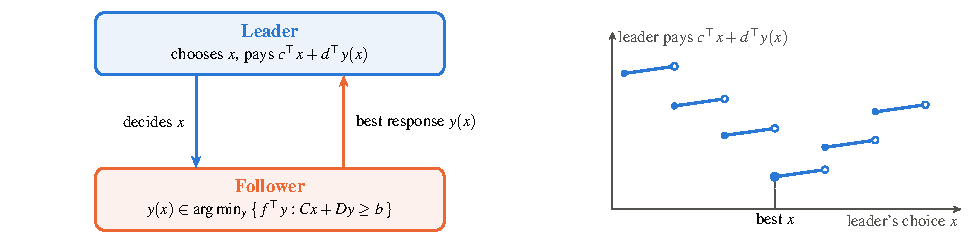
\includegraphics{figures/fig_bilevel_game}
\caption{The bilevel game. The leader chooses $x$ and pays $c\T x+d\T y(x)$, where $y(x)$ is
the follower's best response to $x$. The leader's cost jumps wherever the follower's answer
changes (right: schematic).}\label{fig:game}
\end{figure}

Benchmark libraries focus research effort. For single-level mixed-integer programming, the Mixed
Integer Programming Library (MIPLIB)\cite{bixby1998miplib,koch2011miplib,gleixner2021miplib}
records for every instance whether it is solved, and its open instances have long been targets
for new methods. BOBILib, the Bilevel Optimization (Benchmark) Instance Library of Th\"urauf,
Kleinert, Ljubi\'c, Ralphs and Schmidt,\cite{thurauf2026bobilib,bobilib_website} plays the same
role for MIBLPs. It collects \NumInstances{} instances from the literature in one file format,
with solution files, a feasibility checker and a status per instance. Its metadata of
18~October~2026 lists \NumBobiOptimal{} instances as optimal, \NumBobiInfeasible{} as infeasible,
\NumBobiFeasible{} as feasible (a point is known, but not proven optimal) and \NumBobiOpen{} as
open (no point is known). The statuses come from runs of two general-purpose bilevel solvers,
MibS\cite{tahernejad2020mibs,mibs_software} and the solver of Fischetti et al.\ in its setting
MIX++, or HC++ where MIX++ does not apply,\cite{fischetti2017new,mixpp_software} each for one hour
on one thread. They were fixed when the instances were collected, and some of the specialized
results discussed below appeared later.

This paper asks a simple question: which of the \NumUnsolved{} feasible or open instances (below,
\emph{unsolved}) can be \emph{settled}, that is, proven optimal or proven to have no bilevel
feasible point, and are there methods that settle many of them at once? The goals of the work
were to:
\begin{itemize}
\item reconcile BOBILib's statuses with the per-instance results published since the instances
were collected;
\item find structure shared by many of the remaining instances, and exploit it with methods that
settle whole families rather than single instances;
\item make every claim checkable by a reader who does not trust my code: verified solution files
in BOBILib's own format, a certificate for every bound, and machine-checked proofs where the
argument is new.
\end{itemize}

The main findings are these (Figure~\ref{fig:overview}).
\begin{itemize}
\item Published work had already solved \NumLitOptimal{} of the \NumUnsolved{} instances:
\NumLitKnapsackMethods{} with methods built for knapsack
interdiction\cite{weninger2025fast,fischetti2019interdiction} and \NumLitLozano{} with the
decision diagrams of Lozano, Bergman and Cire.\cite{lozano2026network} Reconciling the statuses
with these results settles more instances than any method of this paper.
\item A new exact search proves all \NumNewKip{} knapsack interdiction instances that were open
in the literature optimal, the slowest in \KipHardestCpu{} seconds. In all of them the optimum
equals the trivial upper bound, so the whole difficulty lies in the lower bound. The main pruning
lemmas of the search are proved in Lean.
\item Two theorems of extremal graph theory, Mantel's and Brouwer's, together with partition
certificates and \NumCliquePartCases{} small cases decided by exact solvers, prove
\NumNewClique{} of the \NumCliqueSet{} edge clique interdiction instances optimal, at values
\CliqueOptSeven{} and \CliqueOptNine{} where BOBILib lists \CliqueBobiMin{} to \CliqueBobiMax{}.
\item In \NumNoFeasible{} instances the follower's problem is infeasible or unbounded for every
leader choice (\NumRayExact{} certificates checked in exact arithmetic), so they have no bilevel
feasible point at all. Another \NumFirstPoint{} instances get a verified point where BOBILib lists
none, \NumFirstAnywhere{} of them the first point anywhere, and \NumOrBetter{} instances of the OR
set a point better than every published one.
\item In total \NumSettled{} (\PctSettled\%) of the \NumUnsolved{} instances are settled,
\NumOptimalNow{} of them optimal: \NumLitOptimal{} by published work and \NumSettledHere{}
(\PctSettledHere\%) by this work. All results are released with an updated status file in MIPLIB's
\code{.solu} format.
\end{itemize}

\begin{figure}[t]
\centering
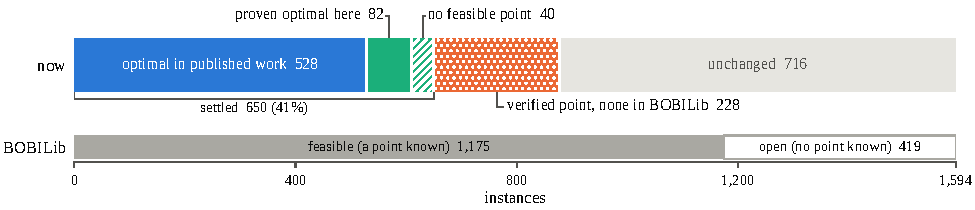
\includegraphics{figures/fig_overview_status}
\caption{Where BOBILib's \NumUnsolved{} feasible or open instances stand. \NumSettled{}
(\PctSettled\%) are settled: \NumLitOptimal{} were already optimal in published work,
\NumNewOptimal{} are proven optimal here and \NumNoFeasible{} have no bilevel feasible point.
Another \NumFirstPoint{} get a verified point where BOBILib lists none (for \NumFirstAnywhere{} of
them the first point anywhere) and \NumUnchanged{} are unchanged. The thin bar shows BOBILib's own
split (\NumBobiFeasible{} feasible, \NumBobiOpen{} open).}\label{fig:overview}
\end{figure}

\textbf{What is new, and what is reused.} New are the reconciliation itself, the robust subset-sum
search with tables rebuilt at every node, the use of Brouwer's stability theorem for edge clique
interdiction, the Lean proofs and the verified data package. The other arguments are known and
are applied here systematically: dualizing the follower's linear programming relaxation into one
mixed-integer program\cite{caprara2016bilevel,wood1993deterministic,israeli2002shortest} and the
integrality gap of a packing problem with few rows, which follows from the fact that a basic LP
solution has at most as many fractional variables as rows;\cite{kellerer2004knapsack} the online lower
bound of Weninger and Fukasawa;\cite{weninger2025fast} Meyer's argument that a rational
mixed-integer program that is feasible and bounded attains its optimum;\cite{meyer1974existence}
the bound $\HPR\le\OPT$ of the high point relaxation;\cite{moore1990mixed} and exhaustive
enumeration.

Section~\ref{sec:background} recalls the problem class and the families in BOBILib.
Section~\ref{sec:methods} describes the methods and how each claim is checked,
Section~\ref{sec:results} gives the computational setup and the results, and
Section~\ref{sec:discussion} discusses why general solvers miss these results, what a benchmark
library could do about it, the limitations of this work and what stays hard. The proofs, the
verification protocol and the per-instance tables are in a separate supplementary document; its
sections are cited as Supp.\ Sec.~A, B, and so on, and its results as, for example, Supp.\ Lemma~B.1.

% ======================================================================================
\section{Background}\label{sec:background}

\subsection{Bilevel Problems in BOBILib Form}

BOBILib writes every instance with a minimizing leader:
\begin{equation}\label{eq:bilevel}
\min_{x,y}\ c\T x+d\T y\quad\text{s.t.}\quad Ax+By\ge a,\qquad
y\in\operatorname*{arg\,min}_{y'}\bigl\{f\T y' : Cx+Dy'\ge b\bigr\},
\end{equation}
with integrality requirements on some of the leader's variables $x$ and the follower's variables
$y$. For a fixed $x$ the follower solves $P(x)=\min\{f\T y: Cx+Dy\ge b\}$ (with its integrality
requirements); $x$ enters it only through the right-hand side. A point $(x,y)$ is \emph{bilevel
feasible} if it satisfies the leader's rows and integrality requirements and $y$ is optimal for
$P(x)$. When the follower has several optimal answers, the one best for the leader is assumed
(the optimistic convention, which BOBILib uses throughout). An upper-level row with a nonzero
coefficient on a follower variable is a \emph{coupling row}; a leader variable that appears in
the follower's rows is a \emph{linking variable}. The \emph{high point relaxation} (HPR) drops the
follower's optimality and keeps every row of both levels,
\[
\HPR=\min\bigl\{c\T x+d\T y : Ax+By\ge a,\ Cx+Dy\ge b,\ \text{integrality}\bigr\},
\]
so $\HPR\le\OPT$, the bilevel optimum.

\subsection{The Families of BOBILib}

Most of BOBILib's unsolved instances are interdiction games: the leader removes parts of the
follower's problem within a budget, and the two objectives are opposite, so the game is
zero-sum and the optimistic and pessimistic readings agree. Table~\ref{tab:families} lists the
families with their outcomes.

\textbf{Packing interdiction.} Items are $N=\{1,\dots,n\}$. The leader chooses $x\in\{0,1\}^n$
within budget rows $Gx\le g$, and the follower packs what is left:
\begin{equation}\label{eq:packing}
\Phi(x)=\max\bigl\{p\T y : Wy\le c,\ y\le \mathbf{1}-x,\ y\in\{0,1\}^n\bigr\},\qquad
\OPT=\min\bigl\{\Phi(x): Gx\le g,\ x\in\{0,1\}^n\bigr\},
\end{equation}
with nonnegative integer profits $p$, weights $W$ and capacities $c$ (from here on, $c$ denotes
capacities, not the cost vector of~\eqref{eq:bilevel}). The knapsack interdiction problem (KIP)
has one leader row, with budget $\beta$, and one follower row, with capacity $c$; the
multidimensional KIP (MKIP) has several of either. In the \emph{subset-sum class} of KIP each
item's profit equals its weight ($p=w$), so the follower's value is the largest sum of surviving
weights that fits the capacity. Figure~\ref{fig:kip} shows a small instance. BOBILib's KIP
instances come from DeNegre,\cite{denegre2011thesis} whose set is built from bicriteria
instances of the Multiple Criteria Decision Making library, and from Caprara, Carvalho, Lodi and
Woeginger\cite{caprara2016bilevel} and Fischetti, Monaci and Sinnl,\cite{fischetti2018dynamic}
whose sets use the item classes of the knapsack generator of Martello, Pisinger and
Toth.\cite{martello1999dynamic} Its MKIP instances form two sets of Fischetti, Ljubi\'c, Monaci
and Sinnl,\cite{fischetti2019interdiction} the \NumImkp{} \emph{imkp} instances built on the
SAC-94 suite\cite{khuri1994zero} and the \NumOr{} \emph{OR} instances built on Chu and Beasley's
multidimensional knapsacks from the OR-Library (Operations Research
Library).\cite{chu1998genetic,beasley1990orlibrary} The OR instances have 100 to 500 items and a
tightness $\alpha\in\{0.25,0.5,0.75\}$: the right-hand side of every knapsack row, the leader's
budget rows and the follower's capacity rows alike, is $\alpha$ times the sum of its coefficients
(below, ``budget 25\%'' means $\alpha=0.25$). They come in three variants: variant \code{-100}
has one follower knapsack, variants \code{-0} and \code{-50} have several.

\begin{figure}[t]
\centering
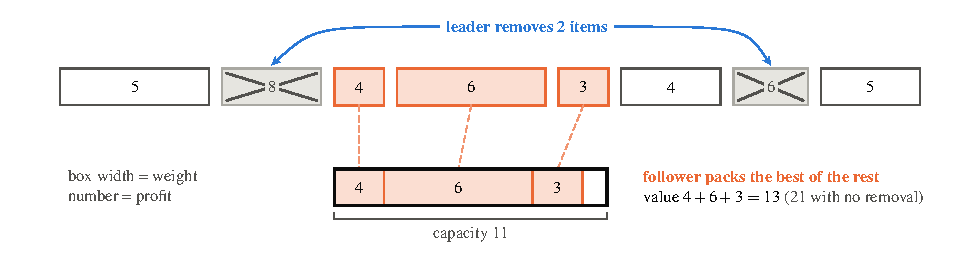
\includegraphics{figures/fig_knapsack_interdiction}
\caption{Knapsack interdiction on a toy instance (box width = weight, number = profit). The
leader removes two items, and the follower packs the best of what is left into its knapsack.
The removal shown cuts the follower's best packing from 21 to 13, and no other pair of removals
does as well.}\label{fig:kip}
\end{figure}

\textbf{Clique interdiction.} The leader deletes a set $D$ of at most $k$ edges of a graph
$G=(V,E)$ with $n$ vertices and $m$ edges, and the follower takes a maximum clique of $G-D$, of
size $\omega(G-D)$. BOBILib's \emph{clique} set of Fischetti, Monaci and
Sinnl\cite{fischetti2018dynamic} has \NumCliqueSet{} instances with $n\in\{40,50,60\}$, edge
density 0.7 or 0.9 and $k=\lfloor m/4\rfloor$; its other clique instances use the graphs of Tang,
Richard and Smith.\cite{tang2016class}

\textbf{Network interdiction.} In the attack-protect game of Baggio, Carvalho, Lodi and
Tramontani\cite{baggio2021multilevel} the leader attacks at most $\Phi$ nodes, the follower then
protects at most $\Lambda$ nodes, and the attack spreads from attacked nodes through unprotected
neighbors. The follower maximizes the number of saved nodes and the leader minimizes it. (Here
$\Phi$ is a budget, as in BOBILib's row names, not the value function of~\eqref{eq:packing}.)

\textbf{General instances.} BOBILib builds most of its general instances from MIPLIB problems,
by assigning the variables and rows to the two levels and keeping the problem's objective as the
leader's.\cite{fischetti2016intersection,fischetti2018intersection,kleinert2021computing} Other
general sets come from DeNegre,\cite{denegre2011thesis} Xu and Wang,\cite{xu2014exact} Ozaltin
and Zhang\cite{ozaltin2017branch} and Fischetti et al.\cite{fischetti2017new} Almost all of the
\NumGeneralUnsolved{} unsolved general instances are MIPLIB-derived; BOBILib lists another
\NumBobiInfeasible{} as infeasible. Generalized interdiction\cite{fischetti2018dynamic} and
assignment interdiction are smaller families.

\begin{table}[t]
\caption{BOBILib's families and the outcome for the instances it lists as feasible or open.
Published: optimal in published work (for \NumLitNoFile{} of them only the published value is
used; Section~\ref{sec:verify}). Here: proven optimal in this work. No point: no bilevel feasible
point exists. New point: a verified bilevel feasible point where BOBILib lists none (for
\NumPointPublishedBefore{} of them a point had been published; Section~\ref{sec:res-overview}).
The total includes BOBILib's \FamAssignmentAll{} assignment interdiction instances, which it lists
as optimal.}\label{tab:families}
\centering\small
\begin{tabular}{@{}l r r r r r r r@{}}
\toprule
 & & Feasible & \multicolumn{5}{c}{Outcome for the feasible or open instances}\\
\cmidrule(l){4-8}
Family & Instances & or open & Published & Here & No point & New point & Unchanged\\
\midrule
Knapsack interdiction (KIP) & \FamKipAll & \FamKipUnsolved & \FamKipLit & \FamKipNew & \FamKipNoFeas & \FamKipFirst & \FamKipUnchanged\\
Multidim.\ knapsack interdiction (MKIP) & \FamMkipAll & \FamMkipUnsolved & \FamMkipLit$^{\dagger}$ & \FamMkipNew & \FamMkipNoFeas & \FamMkipFirst & \FamMkipUnchanged\\
Edge clique interdiction & \FamCliqueAll & \FamCliqueUnsolved & \FamCliqueLit & \FamCliqueNew & \FamCliqueNoFeas & \FamCliqueFirst & \FamCliqueUnchanged\\
Network interdiction & \FamNetworkAll & \FamNetworkUnsolved & \FamNetworkLit & \FamNetworkNew & \FamNetworkNoFeas & \FamNetworkFirst & \FamNetworkUnchanged\\
Generalized interdiction & \FamGeneralizedAll & \FamGeneralizedUnsolved & \FamGeneralizedLit & \FamGeneralizedNew & \FamGeneralizedNoFeas & \FamGeneralizedFirst & \FamGeneralizedUnchanged\\
General, pure integer & \FamGenPureAll & \FamGenPureUnsolved & \FamGenPureLit & \FamGenPureNew & \FamGenPureNoFeas & \FamGenPureFirst & \FamGenPureUnchanged\\
General, mixed integer & \FamGenMixedAll & \FamGenMixedUnsolved & \FamGenMixedLit & \FamGenMixedNew & \FamGenMixedNoFeas & \FamGenMixedFirst & \FamGenMixedUnchanged\\
\midrule
Total & \NumInstances & \NumUnsolved & \NumLitOptimal & \NumNewOptimal & \NumNoFeasible & \NumFirstPoint & \NumUnchanged\\
\bottomrule
\multicolumn{8}{@{}l}{\footnotesize $^{\dagger}$Includes \inst{\OrClosureName}, whose published lower bound is
inconsistent but whose published branch-and-cut bound closes it (Section~\ref{sec:res-or}).}
\end{tabular}
\end{table}

\subsection{What the Literature Had Solved}

\textbf{Knapsack interdiction.} Caprara, Carvalho, Lodi and Woeginger\cite{caprara2016bilevel} gave
an exact algorithm for KIP, and Della Croce and Scatamacchia\cite{dellacroce2020exact}
improved on it. Weninger and Fukasawa's combinatorial branch and
bound\cite{weninger2023fast,weninger2025fast} is the state of the art: it solves \NumKipFiles{} of
BOBILib's \NumKipInstances{} KIP instances, \NumLitKip{} of which BOBILib does not list as optimal.
The \NumNewKip{} instances it leaves open, in runs with 16 threads and a one-hour limit, have
\KipOpenItemsMin{} to \KipOpenItemsMax{} items, and in all of them each profit equals its weight:
\NumKipSubsetSum{} are in the subset-sum class of the generator (class~6) and \NumKipEvenOdd{} in
its even-odd class (class~7: even weights, odd capacity). Their reimplementation of Della Croce
and Scatamacchia's algorithm and two-hour runs of Lozano, Bergman and Cire's decision
diagrams\cite{lozano2026network,lozano_dbo_repo} leave them open too; Weninger and Fukasawa's
published run records\cite{weninger_bkpsolver} give lower bounds \KipPubLbGapMin{} to
\KipPubLbGapMax{} units below BOBILib's values. In every one of these instances BOBILib's value
equals the follower's capacity $c$ (class~6) or $c-1$ (class~7, where every subset sum is even
and $c$ is odd), a trivial upper bound on the follower's value under any leader choice. So the
open question was only the lower bound: can the leader keep the follower from filling its
knapsack exactly (up to parity)?

\textbf{Multidimensional knapsack interdiction.} Fischetti et al.\ solved all \NumImkp{} imkp
instances with interdiction cuts;\cite{fischetti2019interdiction} BOBILib lists \NumLitImkp{} of
them as only feasible, with values up to \ImkpBobiExcessMax\% above the optimum. No OR instance is
optimal in BOBILib. Lozano, Bergman and Cire\cite{lozano2026network} proved \NumLitOr{} of them
optimal and published lower bounds and points for most of the
others,\cite{lozano_dbo_repo} and Lefebvre and Schmidt\cite{lefebvre2025dantzig} published
further points; \NumOrNoPublished{} OR instances had no published point.

\textbf{Clique, network and general instances.} Furini et al.\ gave exact algorithms for vertex and
edge clique interdiction,\cite{furini2019maximum,furini2021branch} but the
\NumCliqueSet{} instances of the clique set had no published optimum. Deciding whether at most $k$
deletions bring the clique number down to a given value is the edge blocker clique
problem.\cite{mahdavipajouh2020minimum} For general MIBLPs the methods are branch and
bound\cite{moore1990mixed} and branch and cut,\cite{denegre2009branch,tahernejad2020mibs}
intersection cuts,\cite{fischetti2016intersection,fischetti2018intersection,fischetti2017new}
value-function reformulations,\cite{mitsos2010global,lozano2017value} decision
diagrams,\cite{lozano2026network,vasquez2025single} a Dantzig--Wolfe single-level
reformulation\cite{lefebvre2025dantzig} and heuristics such as a penalty alternating direction
method (PADM).\cite{kleinert2021computing} Published work solves \NumLitMiplib{} MIPLIB-derived
instances that BOBILib does not list as optimal: \NumLitMiplibLozano{} by Lozano et al.;
\inst{air03-0.100000} by Fischetti et al.;\cite{fischetti2017new} \inst{p0282-0.500000} by
V\'asquez, Lozano and van Hoeve;\cite{vasquez2025single} and \inst{neos-950242\_0\_100}, which an
earlier BOBILib release listed as optimal and whose BOBILib point also meets the MIPLIB bound of
Section~\ref{sec:general} (Supp.\ Table~S11). Lozano et al.\ also solve \NumLitGeneralized{}
generalized interdiction instances.

% ======================================================================================
\section{Methods}\label{sec:methods}

\subsection{Reconciling the Statuses and Verifying Every Claim}\label{sec:verify}

\textbf{Published results.} For every family I compared BOBILib's status and value with the
per-instance data the authors publish: Weninger and Fukasawa's answer files and run
records,\cite{weninger_bkpsolver} the tables of Fischetti et al., the solution files of Lozano,
Bergman and Cire,\cite{lozano_dbo_repo} the run files of Lefebvre and
Schmidt,\cite{lefebvre2025dantzig} and the other papers cited above. An instance counts as solved
in published work only when a proven optimal value is published for it. Each KIP instance was
matched to Weninger and Fukasawa's file by its capacities and the multiset of item triples
(profit, follower weight, leader cost); every match is unique. For \NumLitWithFile{} of the
\NumLitOptimal{} published optima a verified solution file at the published optimum is in the data
package: for all \NumLitKip{} KIP instances it was rebuilt from Weninger and Fukasawa's leader
choices, and for \NumOrLitOptimalPoint{} of the \NumLitOr{} OR instances this work's own point has
the published value. For the other \NumLitNoFile{} (\NumLitNoFileImkp{} imkp,
\NumLitNoFileOr{} OR, \NumLitNoFileMiplib{} MIPLIB-derived and \NumLitNoFileGeneralized{}
generalized interdiction instances) only the published value is used. At \NumKipBobiAbove{} of
the KIP instances BOBILib's value is above the optimum, by a median of \KipBobiExcessMedian\% and
up to \KipBobiExcessMax\%. The literature's optimality proofs are not repeated here.

\textbf{Verification.} Every solution file of this work uses BOBILib's format and passes
\code{bobi verify}, a verifier written for this work after BOBILib's own feasibility checker
(\supp{A.2}). It is separate from BOBILib's solvers, but not from the rest of this work's code: it
shares the instance reader and the exact knapsack oracle with the solvers. It checks (a)~every
row, bound and integrality requirement of the HPR at the file's point; (b)~the stated leader
objective; and (c)~follower optimality: with the leader's variables fixed, the follower's problem
is solved again, with one follower row by an exact knapsack oracle, a branch and bound with
Dantzig's linear programming (LP) bound that falls back to dynamic
programming,\cite{dantzig1957discrete,martello1990knapsack} and otherwise as a mixed-integer
linear program (MILP) with HiGHS.\cite{huangfu2018parallelizing} The file's follower value
$\varphi_{\mathrm{sol}}$ must pass BOBILib's relative test against the proven optimum
$\varphi_{\mathrm{check}}$,
\begin{equation}\label{eq:tol}
\frac{|\varphi_{\mathrm{sol}}-\varphi_{\mathrm{check}}|}{10^{-10}+|\varphi_{\mathrm{check}}|}\le 10^{-4}.
\end{equation}
Table~\ref{tab:tol} collects the tolerances used here and by BOBILib's checker. Code that shares
nothing with the solvers re-checks the knapsack interdiction lower bounds, the recession
directions and the HPR comparisons (Section~\ref{sec:lean}). In this paper ``optimal'' means a
bilevel feasible point in this sense whose value equals a proven lower bound, or, for the
\NumLitNoFile{} published optima without a solution file here, the published claim. Each lower
bound of this work is a theorem with a published certificate, an exact search, an exhaustive
enumeration or, for one OR instance, a published bound, as described below. The full protocol is in \supp{A.3}.

\begin{table}[t]
\caption{Tolerances of the checks.}\label{tab:tol}
\centering\small
\begin{tabular}{@{}>{\raggedright\arraybackslash}p{4.6in} l@{}}
\toprule
Check & Tolerance\\
\midrule
\code{bobi verify}: rows, bounds and integrality of the HPR at a file's point & $10^{-6}$ absolute\\
\code{bobi verify}: follower optimality, test~\eqref{eq:tol} (differences up to $10^{-9}$ count as zero) & $10^{-4}$ relative\\
\code{bobi certify} (points with coupling rows): follower optimality and optimistic tie-break, by proven dual bounds & $10^{-5}$ relative\\
Best response inside \code{bobi general} and \code{bobi coupled}: follower value above its optimum & $10^{-7}(1+|\varphi|)$\\
BOBILib's checker: rows and integrality (MIPLIB solution checker) & $10^{-4}$\\
BOBILib's checker: follower optimality, test~\eqref{eq:tol} & $10^{-4}$ relative\\
\bottomrule
\end{tabular}
\end{table}

\subsection{Knapsack Interdiction: A Robust Subset-Sum Search}\label{sec:kip}

All \NumNewKip{} KIP instances open in the literature are subset-sum instances: the follower's
value is the largest sum of surviving weights that fits its capacity. The search answers a
yes/no question: given an integer $\ell$, does every leader choice within budget leave the
follower a subset sum in the band $[\ell,c]$? A ``yes'' proves $\OPT\ge\ell$; a ``no'' comes with
a leader choice whose follower value is below $\ell$. The loop starts from Weninger and
Fukasawa's greedy leader choice and asks the question with $\ell$ equal to the value of the best
leader choice found so far; it stops at the first ``yes'', which proves optimality (Supp.\
Cor.~B.25). For each of the \NumNewKip{} instances it stopped at BOBILib's value, $c$ or $c-1$, so
the band $[\ell,c]$ has width 0 or 1. The rules below hold for any band; for an instance whose
optimum lies far below $c$ the band is wider, and the loop may need several searches.

\textbf{Count formulation.} Subset-sum instances have many items with the same weight. Such items
are interchangeable for the follower, so the leader should delete the cheapest copies first,
and the search branches on how many copies of each weight survive rather than on which items
are deleted (Figure~\ref{fig:ss}a; Supp.\ Prop.~B.4, which also divides the weights by their
greatest common divisor). This removes many symmetric branches.

\begin{lem}[Monotonicity and cheapest copies]\label{lem:count}
(i) Blocking more items never helps the follower: $X\subseteq X'$ implies $\Phi(X')\le\Phi(X)$.
(ii) For a class $Q$ of identical items and any leader set $X$ there is a leader set $X'$ that
agrees with $X$ outside $Q$, blocks as many copies of $Q$, blocks only copies no costlier than
every copy it leaves, costs no more than $X$, and has $\Phi(X')=\Phi(X)$.
\end{lem}
\noindent Proof in Supp.\ Lemmas~B.1 and~B.2; Lean: \lean{follower\_antitone},
\lean{cheapest\_first}.

\textbf{Windows.} At a node of the search the decided classes have left survivors $M$ whose subset
sums are known. A run of consecutive reachable sums only grows when a copy of value $v$ is added,
as long as $v$ is at most the run's width (Figure~\ref{fig:ss}b; Lean: \lean{window\_extend},
\lean{window\_extend\_all}). If the leader cannot afford to delete enough weight to stop such a
window before it reaches the band, the node is safe whatever the leader does (Supp.\
Prop.~B.8).

\textbf{The online game.} The strongest rule is an online relaxation due to Weninger and
Fukasawa. Fix an order of the items. In the online game the leader decides item by item whether
to block it, and the follower, who has seen every earlier move, decides whether to take each
unblocked item. The leader may react to the follower's earlier choices, which it cannot do in
the real game, so the follower's value in the online game is a lower bound:

\begin{thm}[Online lower bound\cite{weninger2025fast}]\label{thm:online}
For every list $o$ of distinct items, the value $\Omega(o,\beta,c)$ of the online game, computed
by backward induction, satisfies $\Omega(o,\beta,c)\le\Phi(X)$ for every leader set $X$ within
the budget $\beta$. Hence $\Omega(o,\beta,c)\le\OPT$.
\end{thm}
\noindent Proof in Supp.\ Thm~B.9; Lean: \lean{online\_le\_K\_any},
\lean{online\_lower\_bound}.

\textbf{Tables with an end set.} For subset-sum instances I play the online game class by class,
in the count formulation and with a target. At each class the leader announces how many copies
it deletes; the follower then takes some of the surviving copies, which lowers a residual $t$;
the follower wins if the final residual lies in an \emph{end set} $A$. Let $G_A(Q,\beta')$ be the
set of residuals from which the follower wins when the classes $Q$ are played in a given order
and the leader has budget $\beta'$. Then every deletion within $\beta'$ leaves a subset sum $s$
with $t-s\in A$ (Supp.\ Thm~B.12; Lean: \lean{GA\_sound}, and \lean{GA\_sound\_perm} for any order
of play). A follower who wins against a budget also wins against any smaller one, so the table is
stored as one number per residual: the largest budget against which the follower still wins.
These thresholds satisfy a min-max recursion over the classes, and one backward pass computes
them for all residuals (Supp.\ Thm~B.17; Lean: \lean{thr\_iff}, \lean{GA\_iff\_thr}).

\begin{figure}[t]
\centering
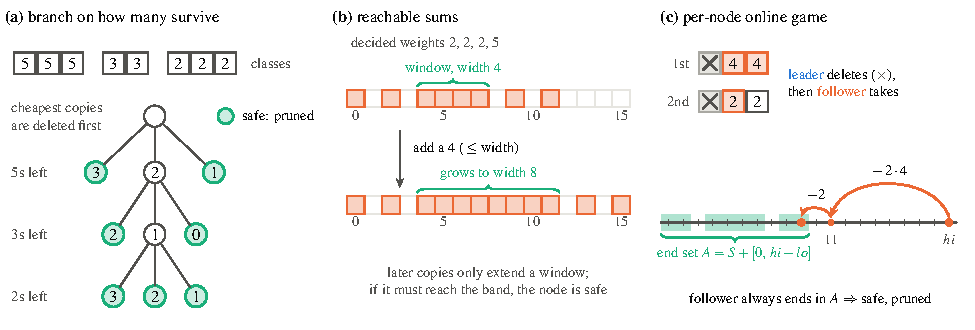
\includegraphics{figures/fig_subset_sum_search}
\caption{The search that proves the \NumNewKip{} new knapsack interdiction optima, on toy
numbers. (a)~It branches on how many copies of each weight survive. (b)~A window of consecutive
reachable sums only grows as copies are added. (c)~At each node an online game, in which the
leader deletes one weight class at a time, decides whether the follower can always end in the
set $A$; if so the node is pruned.}\label{fig:ss}
\end{figure}

\textbf{The per-node rule.} The decided survivors at a node already reach a set $S$ of subset sums,
and the follower wins with any total in $[\ell,c]$. So the node's end set is
$A_{\mathrm{node}}=\{a\in[0,c]: s\le a\le s+(c-\ell)\text{ for some }s\in S\}$, and the game starts
from the residual $c$: if it ends at $a\in A_{\mathrm{node}}$, the follower's total $c-a$ plus a
suitable $s\in S$ lies in the band.

\begin{thm}[Per-node rule]\label{thm:node}
At a node with decided sums $S$ and residual budget $\beta'$, let $\pi$ be any order of the
undecided classes. If $\beta'$ is at most the threshold of the residual $c$ in the table for
$\pi$ with end set $A_{\mathrm{node}}$, then every completion of the node within $\beta'$ leaves
a subset sum in $[\ell,c]$: the node can be pruned, and it stays safe for every smaller budget.
\end{thm}
\noindent Proof in Supp.\ Thm~B.19; Lean: \lean{node\_table\_sound\_perm} and
\lean{node\_table\_threshold\_sound\_counts}.

Figure~\ref{fig:ss}c shows the rule on toy numbers. The decided sums are $S=\{0,3,5,8\}$ and the
band is $[18,19]$, so $A_{\mathrm{node}}=\{0,1,3,4,5,6,8,9\}$. Three copies of 4 and three of 2
are undecided, each copy costs 1 to delete, and the leader has budget 2. The game starts at the
residual 19. In the play shown, the leader deletes a 4 and the follower takes the other two
(residual 11); the leader deletes a 2 and the follower takes one of the two left (residual
$9\in A_{\mathrm{node}}$). The follower's total $8+2=10$ plus $s=8$ is 18, in the band. Checking
every play shows that the follower can always end in $A_{\mathrm{node}}$ at budget 2, so the node
is pruned.

The table is rebuilt from the node's own sums at every node that would otherwise branch, and
its threshold is cached, so later nodes with the same depth and sums and a budget below the
threshold are pruned at once. The search also uses cheaper rules: the \emph{direct} rule (the
decided sums $S$ already meet $[\ell,c]$), guaranteed copies, the window rule and the cache (Supp.\
Thm~B.23). The order of play does not affect soundness but matters a great deal for strength. The
search plays the classes that are cheapest to delete per unit of weight first: the follower then
sees the leader's likely deletions before it commits, and keeps the expensive classes for fine
adjustment. On \inst{interKP-200-100-6-2}, tables built only at the root needed
\KipAblationLargestFirst{} nodes when played largest weight first and \KipAblationCheapestFirst{}
when played cheapest first; per-node tables need \KipAfterNodesTwoSixTwo{}. A node is declared
``blocking'' only at a leaf no rule prunes, which yields a leader choice below $\ell$; so a search
that ends within its node limit is exact (Supp.\ Thm~B.24).

\subsection{Multidimensional Knapsack Interdiction: A Linear Programming Bracket}\label{sec:mkip}

Let $U(x)$ be the value of the follower's LP relaxation in~\eqref{eq:packing},
in which the follower may take fractions of items, and $\pmax$ the largest profit. Dualizing the
follower's LP gives
\[
U(x)=\min_{\lambda\ge 0}\ c\T\lambda+\sum_{j=1}^n\max\bigl(0,\,p_j-(W\T\lambda)_j\bigr)(1-x_j),
\]
and for binary $x$ the product linearizes exactly, so $U^*=\min\{U(x): Gx\le g\}$ is the value of
a single MILP (Supp.\ Prop.~C.2). Caprara et al.'s algorithm for KIP rests on this
dualization,\cite{caprara2016bilevel,dellacroce2020exact} and it is the classical single-level
reformulation of network interdiction.\cite{wood1993deterministic,israeli2002shortest} An optimal vertex of the follower's
LP has at most $m$ fractional items when the follower has $m$ rows, which bounds the gap between
$U$ and $\Phi$ (Figure~\ref{fig:bracket}).

\needspace{6\baselineskip}
\begin{thm}[LP bracket]\label{thm:bracket}
With $m$ follower rows, $U(x)-m\,\pmax\le\Phi(x)\le U(x)$ for every leader choice $x$. Hence for
any lower bound $L\le U^*$, for example a MILP solver's proven dual bound, and any leader-feasible
$\hat x$:\ \ $\lceil L-m\,\pmax\rceil\le\OPT\le\Phi(\hat x)\le U(\hat x)$.
\end{thm}
\noindent Proof in Supp.\ Lemma~C.3 and Thm~C.4; not formalized.

\begin{figure}[t]
\centering
\begin{minipage}[c]{0.5\textwidth}
\centering
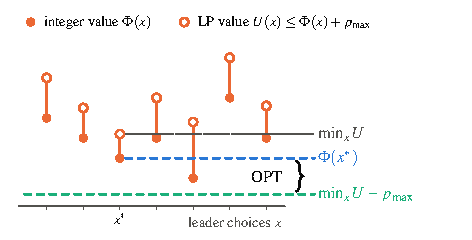
\includegraphics{figures/fig_lp_bracket}
\end{minipage}\hfill
\begin{minipage}[c]{0.46\textwidth}
\caption{The LP bracket for one follower knapsack (made-up numbers): the follower's LP value
$U(x)$ exceeds its integer value $\Phi(x)$ by at most $\pmax$, so the optimum lies between
$\min_x U-\pmax$ and $\Phi(\hat x)$, where $\hat x$ minimizes $U$.}\label{fig:bracket}
\end{minipage}
\end{figure}

With one follower knapsack (variant \code{-100}, $m=1$) the bracket is at most one item's profit
wide when the MILP is solved to optimality ($L=U^*$ at its minimizer $\hat x$); with a time limit
its width is $\Phi(\hat x)-\lceil L-\pmax\rceil$. A second lower bound extends
Theorem~\ref{thm:online} to several leader rows: merge them into one row with nonnegative
multipliers, then round the leader's costs down and its budget up, and the follower's weights up
and its capacity down. Each step only helps the leader, so the online game on the merged data is
still a lower bound (Supp.\ Thm~C.5; the online bound is formalized, the merging and rounding are
not). Upper bounds come from a first-improvement local search on the leader's choice that
evaluates each candidate with the exact knapsack oracle, so every point it reports is certified.

With several follower knapsacks (variants \code{-0} and \code{-50}) the bracket's width
$m\,\pmax$ is too large for a useful lower bound, and only the literature's lower bounds are used.
The minimizer $\hat x$ of the MILP is still a good leader choice: whenever HiGHS solves the
follower's integer problem at $\hat x$ to proven optimality, the point is certified (\supp{C.4}).

\subsection{Clique Interdiction: Extremal Graph Theory and Partitions}\label{sec:clique}

After any deletion at least $m-k$ edges remain, and extremal graph theory says how many edges
force a clique of a given size.

\begin{thm}[Clique bounds]\label{thm:clique}
Let $G$ have $n$ vertices and $m$ edges, and let the leader delete at most $k$ edges.
\begin{enumerate}
\item[(i)] (Mantel\cite{mantel1907problem}) If $m-k>\lfloor n^2/4\rfloor$, every remainder contains
a triangle, so the value is at least~3.
\item[(ii)] (Partitions) If the vertices can be split into $r$ parts with at most $k$ edges
inside the parts, deleting those edges leaves an $r$-partite graph, so the value is at most~$r$.
\item[(iii)] (Brouwer\cite{brouwer1981lotto,tyomkyn2015strong}) If $n\ge 7$,
$m-k\ge t_3(n)-\lfloor n/3\rfloor+2$, and every split of the vertices into 3 parts has more than
$k$ edges inside the parts, every remainder contains a $K_4$, so the value is at least~4.
\end{enumerate}
\end{thm}
\noindent Proof in Supp.\ Thms~D.2 and~D.6 and Prop.~D.3. Parts (i) and (ii) are proved in Lean
(\lean{mantel}, \lean{triangle\_survives} and \lean{cliqueFree\_of\_partition}); part~(iii) is
not formalized, as it rests on Brouwer's theorem.

Here $t_3(n)$ is the number of edges of the balanced complete 3-partite graph on $n$ vertices,
the Tur\'an number.\cite{turan1941extremal} Brouwer's Theorem~2 of 1981, in an unrefereed
report,\cite{brouwer1981lotto} says that a $K_4$-free graph on $n\ge 7$ vertices with at least
$t_3(n)-\lfloor n/3\rfloor+2$ edges is 3-partite. Tyomkyn and Uzzell give a new proof of this
statement in a refereed journal (their Theorem~1.1, for $K_{r+1}$-free graphs; here
$r=3$).\cite{tyomkyn2015strong} It was also found again by Hanson and Toft and by Kang and
Pikhurko,\cite{hanson1991ksaturated,kang2005maximum} and Amin, Faudree, Gould and Sidorowicz
determine the largest number of edges of a maximal $K_p$-free graph that is not $(p-1)$-partite,
which for $p=4$ gives the same threshold.\cite{amin2013non} So in (iii) a $K_4$-free remainder
would be 3-partite, the deletion would contain every edge inside the parts of some 3-partition,
and that takes more than $k$ deletions. Table~\ref{tab:clique} gives the numbers. At density 0.7
Mantel's theorem applies. At density 0.9 Brouwer's threshold is met, while $m-k$ stays below
$t_3(n)$, so Tur\'an's theorem alone would not give a $K_4$. Figure~\ref{fig:clique} shows the
argument on a small graph.

\begin{table}[t]
\caption{Edge counts behind the clique lower bounds. Every instance of a group has the same $n$,
$m$ and $k$. Mantel's theorem needs $m-k>\lfloor n^2/4\rfloor$; Brouwer's needs
$m-k\ge t_3(n)-\lfloor n/3\rfloor+2$.}\label{tab:clique}
\centering\small
\begin{tabular}{@{}r c r r r r r r c@{}}
\toprule
$n$ & Density & $m$ & $k$ & $m-k$ & $\lfloor n^2/4\rfloor$ & $t_3(n)$ & $t_3(n)-\lfloor n/3\rfloor+2$ & Optimum\\
\midrule
40 & 0.7 & \CliqueMFortySeven & \CliqueKFortySeven & \CliqueMantelLhsForty & \CliqueMantelRhsForty & \CliqueTuranForty & \CliqueBrouwerRhsForty & \CliqueOptSeven\\
50 & 0.7 & \CliqueMFiftySeven & \CliqueKFiftySeven & \CliqueMantelLhsFifty & \CliqueMantelRhsFifty & \CliqueTuranFifty & \CliqueBrouwerRhsFifty & \CliqueOptSeven\\
60 & 0.7 & \CliqueMSixtySeven & \CliqueKSixtySeven & \CliqueMantelLhsSixty & \CliqueMantelRhsSixty & \CliqueTuranSixty & \CliqueBrouwerRhsSixty & \CliqueOptSeven$^{*}$\\
40 & 0.9 & \CliqueMFortyNine & \CliqueKFortyNine & \CliqueBrouwerLhsForty & \CliqueMantelRhsForty & \CliqueTuranForty & \CliqueBrouwerRhsForty & \CliqueOptNine\\
50 & 0.9 & \CliqueMFiftyNine & \CliqueKFiftyNine & \CliqueBrouwerLhsFifty & \CliqueMantelRhsFifty & \CliqueTuranFifty & \CliqueBrouwerRhsFifty & \CliqueOptNine\\
60 & 0.9 & \CliqueMSixtyNine & \CliqueKSixtyNine & \CliqueBrouwerLhsSixty & \CliqueMantelRhsSixty & \CliqueTuranSixty & \CliqueBrouwerRhsSixty & \CliqueOptNine\\
\bottomrule
\multicolumn{9}{@{}l}{\footnotesize $^{*}$\,Except three instances of this group, which are open,
with value \CliqueOpenLower{} or \CliqueOpenUpper{} (Section~\ref{sec:res-clique}).}
\end{tabular}
\end{table}

The last condition of (iii) reduces to finitely many cases. Counting the non-edges inside the
parts, a 3-partition with given part sizes has few edges inside its parts exactly when few
edges of the sparse complement graph join different parts. Only a handful of part-size vectors
leave any room, and for each of them a partition with at most $k$ inside edges would need at most
a few complement edges between the parts (Supp.\ Prop.~D.7). That gives
\NumCliquePartCases{} cases (instance, part sizes), each decided infeasible by several methods:
CP-SAT\cite{perron2026cpsat} and SCIP\cite{hojny2025scip,maher2016pyscipopt} on two different
models, an exact depth-first search that uses no solver, and, in a separate review session with
its own code, HiGHS on a third model and a branch and bound written in C. These verdicts are
computations, not formal proofs. For the upper bounds, a tabu search looks for 3- and
4-partitions with few inside edges. Each solution file deletes exactly the inside edges of a
partition and states a maximum clique of the remainder, computed exactly and checked again with
two exact clique searches.\cite{bron1973algorithm,tomita2006worst,carraghan1990exact}

\begin{figure}[t]
\centering
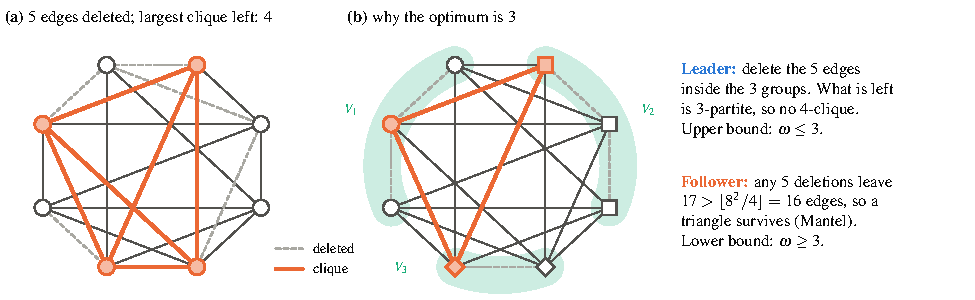
\includegraphics{figures/fig_clique_interdiction}
\caption{Clique interdiction on an 8-vertex graph with budget 5. (a)~A deletion that still
leaves a 4-clique. (b)~Why the optimum is 3: deleting the 5 edges inside the groups $V_1$ to
$V_3$ leaves a 3-partite graph, so no 4-clique survives (Theorem~\ref{thm:clique}(ii)), and any 5
deletions leave more than $\lfloor 8^2/4\rfloor$ edges, so a triangle survives
(Theorem~\ref{thm:clique}(i)).}\label{fig:clique}
\end{figure}

\subsection{Network Interdiction: Every Attack, with an Exact Tree Program}\label{sec:network}

For a fixed attack, the follower's best response in the attack-protect game is a closure problem:
the burned nodes are the smallest set that contains the attacked nodes and is closed under
spreading to unprotected neighbors (Supp.\ Lemma~F.1). On a forest it is solved exactly by a
dynamic program (DP) over the states (protected, saved) of each node, with the number of
protected nodes as a knapsack dimension (\supp{F.3}). The two instances BOBILib lists as
feasible are forests with \NetworkNodes{} nodes and $\Phi=\Lambda=\NetworkPhi$, so all
\NetworkAttacks{} attacks of at most $\Phi$ nodes can be enumerated (Figure~\ref{fig:network}).
Every follower point is checked against the model as read from the files, and at the minimizing
attack the follower's MILP is solved again by HiGHS. The minimum over all attacks is then the
optimum (Supp.\ Thm~F.4).

\begin{figure}[t]
\centering
\begin{minipage}[b]{0.47\textwidth}
\centering
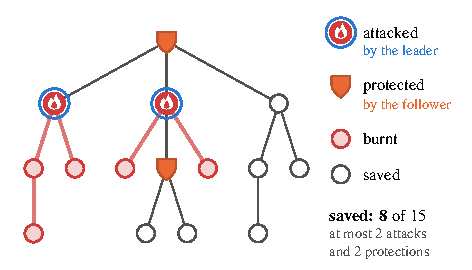
\includegraphics{figures/fig_network_attack_protect}
\end{minipage}\hfill
\begin{minipage}[b]{0.47\textwidth}
\centering
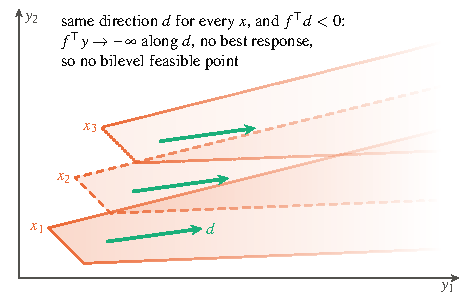
\includegraphics{figures/fig_unbounded_follower}
\end{minipage}\par\vspace{4pt}
\begin{minipage}[t]{0.47\textwidth}
\caption{The attack-protect game on a toy tree: the leader attacks, the follower then
protects, and the attack spreads through unprotected neighbors. Against the optimal attack
shown, the follower saves at most the nodes marked as saved.}\label{fig:network}
\end{minipage}\hfill
\begin{minipage}[t]{0.47\textwidth}
\caption{Why some MIPLIB-derived instances have no bilevel feasible point: the follower's region
moves with the leader's choice $x$ but keeps the same direction $r$, and $f\T r<0$ leaves the
follower without a best response for every $x$.}\label{fig:ray}
\end{minipage}
\end{figure}

\subsection{General Instances: Recession Directions, the MIPLIB Bound and Feasible Points}\label{sec:general}

\textbf{No bilevel feasible point.} The leader's variables enter the follower's rows only as
constants. So a direction along which the follower can improve without limit works for every
leader choice at once (Figure~\ref{fig:ray}).

\needspace{7\baselineskip}
\begin{thm}[Recession direction]\label{thm:ray}
Let $r$ be a rational direction of the follower's variables that keeps every follower row and
bound satisfied when added to a feasible point ($D_ir\ge 0$ for a row with a finite lower side,
$D_ir\le 0$ for a row with a finite upper side, and the same sign conditions for the variable
bounds), and let $f\T r<0$. Then for every leader choice the follower's problem is infeasible or
unbounded, so the bilevel problem has no feasible point.
\end{thm}
\noindent Proof in Supp.\ Thm~E.1, after Meyer;\cite{meyer1974existence} not formalized.

The integrality of the follower is no obstacle because $r$ is rational: a multiple of $r$ keeps
the integer variables integral. The directions are found by an LP solver in floating point. A
script that reads the instance files independently of the solver code converts each direction
to exact rationals and checks the conditions of Theorem~\ref{thm:ray} in rational arithmetic.

\textbf{The MIPLIB bound.} Every bilevel feasible point is feasible for the HPR, so $\HPR\le\OPT$,
and a bilevel feasible point with value $\HPR$ is optimal (Supp.\ Lemma~E.3). When BOBILib
builds an instance from a MIPLIB problem and changes nothing else, the HPR \emph{is} that MIPLIB
problem, and its published optimum\cite{gleixner2021miplib} is a lower bound on the bilevel
optimum. This is checked, not assumed: a script compares the bilevel
instance with the MIPLIB~2017 model in exact rational arithmetic (variables, rows, coefficients,
sides, bounds, integrality and objective).


\textbf{Feasible points.} Without coupling rows, a bilevel feasible point follows from any HPR
point at which the follower's problem has an optimal solution: fix the leader's part, solve the
follower to optimality, and choose among the follower's optima the one best for the leader, the
optimistic tie-break (Supp.\ Prop.~E.4). Unlike BOBILib's two solvers, this handles continuous
linking variables. With coupling rows, all follower optima at the HPR's leader values may violate
a coupling row. For fixed values of the linking variables at which the follower's problem has an
optimum, two solves, the follower's problem and then one MILP for the optimistic best response
with the coupling rows, find the best bilevel feasible point with those values or show that there
is none (Supp.\ Prop.~E.5). A portfolio of heuristics, \code{bobi coupled}, searches for usable
linking values: the HPR's own values, best-response dynamics, an HPR whose objective is penalized
by the follower's, PADM,\cite{kleinert2021computing} moves of continuous linking variables into
the interior, value-function cuts\cite{mitsos2010global,lozano2017value} and no-good cuts. None
of these is needed for correctness. What is certified is each returned point, checked again from
scratch with proven dual bounds on the follower's problem and on the optimistic tie-break
(Table~\ref{tab:tol}), and then by \code{bobi verify}.

\subsection{Formal Verification and Separate Checks}\label{sec:lean}

The main lemmas behind the new exact search and the clique bounds are proved in the Lean~4
theorem prover\cite{moura2021lean} with its mathematical library Mathlib\cite{mathlib2020}
(Table~\ref{tab:lean}). The project contains no \code{sorry}, and every main theorem uses only
Lean's standard axioms (\code{propext}, \code{Classical.choice} and \code{Quot.sound}). The Lean
statements are about abstract models (items, weight classes, graphs), not about the Rust code:
that the code computes the formalized recursions is argued in its documentation and tested
against brute force, not proved. The full map from results to Lean theorems and to the code that
relies on them is in \supp{G}.

\begin{table}[t]
\caption{What is machine-checked. Lean theorem names are in the namespace \code{Bobi} of the
project \code{bobilib/lean}; Supp.: section of the supplementary document.}\label{tab:lean}
\centering\small
\begin{tabular}{@{}>{\raggedright\arraybackslash}p{2.05in}>{\raggedright\arraybackslash}p{3.65in}>{\raggedright\arraybackslash}p{0.5in}@{}}
\toprule
Result & Lean theorems & Supp.\\
\midrule
Monotonicity, cheapest copies first (Lemma~\ref{lem:count}) & \lean{follower\_antitone}, \lean{cheapest\_first} & B.1\\
Windows of reachable sums & \lean{window\_extend(\_all)}, \lean{window\_survivors} & B.2\\
Online lower bound (Theorem~\ref{thm:online}) & \lean{online\_lower\_bound}, \lean{online\_le\_K\_any} & B.3\\
Tables with an end set, any order of play & \lean{H\_sound(\_any)}, \lean{G\_sound}, \lean{GA\_sound}, \lean{GA\_sound\_perm},\newline \lean{covers\_sound}, \lean{band\_covers\_sound} & B.4\\
Threshold form & \lean{thr\_iff}, \lean{GA\_iff\_thr}, \lean{covers\_threshold\_sound(\_perm)},\newline \lean{band\_covers\_threshold\_sound(\_perm)} & B.5\\
Per-node rule (Theorem~\ref{thm:node}) & \lean{node\_table\_sound}, \lean{node\_table\_sound\_perm},\newline \lean{node\_table\_threshold\_sound\_counts} & B.6\\
Mantel's theorem, deletion form (Theorem~\ref{thm:clique}(i)) & \lean{mantel}, \lean{triangle\_survives} & D.2\\
Partition upper bound (Theorem~\ref{thm:clique}(ii)) & \lean{cliqueFree\_of\_partition} & D.3\\
\midrule
\multicolumn{3}{@{}p{6.5in}@{}}{\raggedright \emph{Not formalized:} the search code itself; the
reduction to the count formulation with its scaling by the greatest common divisor (Supp.\
Prop.~B.4); the fractional deletion bound in the window rule; the direct, guaranteed-copies and
cache rules and the node-state lemma (Supp.\ Thm~B.23 and Lemma~B.22); restricted copies (an
option no recorded run uses); the LP bracket and the merged-row bound; Brouwer's theorem and the
part-size verdicts; the network DP; the recession directions and the MIPLIB comparison.}\\
\bottomrule
\end{tabular}
\end{table}

\textbf{Separate checks.} The software, the experiments and the checks below were carried out with
an AI coding agent directed by the author (see the Acknowledgements). The checks described as
separate reviews ran in fresh sessions of the same agent that wrote their own code and their own
instance readers, without reading the code they checked; they are separate re-implementations,
not independent human reviews. The \NumNewKip{} subset-sum lower bounds were proved again by two
Python provers that share no code with the Rust search: one written with the search, the other in
a separate review session. Both parse the instance files themselves and use only the direct rule
and the per-node rule, in integer arithmetic. Two other designs of the search, built separately,
prove \inst{interKP-200-100-6-3}, and every search binary was compared with exhaustive
enumeration on \KipBruteForceInstances{} random small instances, with
\KipBruteForceMismatches{} mismatches. The clique, network and coupled-row results were each
derived again in a separate review session with its own instance reader and different solvers or
code: two exact maximum-clique searches, HiGHS and a branch and bound in C for the part-size cases;
a C implementation of the tree DP compared with ours at every attack; and a second reading of the
coupled files with HiGHS's own reader. The reviews' notes and their corrections are in the
\code{README} files of the data package; Section~\ref{sec:limits} discusses the risk of errors
that all these checks share.

% ======================================================================================
\section{Results}\label{sec:results}

\subsection{Computational Setup}\label{sec:setup}

The computations ran on a virtual machine with four cores of an Intel Xeon processor at 2.1~GHz
and 15~GB of memory (Ubuntu 24.04; Rust 1.97; Python 3.13; HiGHS 1.15, SCIP 10.0 through
PySCIPOpt 6.3, CP-SAT 9.15; Lean 4.35 with Mathlib). The machine was shared with other jobs and
often oversubscribed. Every method ran on one thread, except CP-SAT, which used two workers.
Table~\ref{tab:setup} lists the runs. An unsolved instance outside them was not attempted; in
particular the general instances that BOBILib lists as feasible were only compared with the
literature and, where their point meets the MIPLIB optimum, with the MIPLIB bound. Times are CPU
seconds where so stated and wall-clock seconds otherwise, and no proof depends on them. The total
computing effort was not recorded; the data package gives per-instance times where measured.

\begin{table}[t]
\caption{Methods, the instances they were run on, their limits per instance, and their outcomes
(Supp.\ Sec.~H and the \code{README} files of the data package give the commands).}\label{tab:setup}
\centering\small\setlength{\tabcolsep}{4pt}
\begin{tabular}{@{}>{\raggedright\arraybackslash}p{1.5in}>{\raggedright\arraybackslash}p{1.65in}>{\raggedright\arraybackslash}p{1.45in}>{\raggedright\arraybackslash}p{1.6in}@{}}
\toprule
Method & Run on & Limits & Outcome\\
\midrule
Robust subset-sum search & the \NumNewKip{} open KIP instances; \NumKipValidation{} with published optima & none reached; every run finished & \NumNewKip{} optimal; all \NumKipValidation{} published optima reproduced\\
LP bracket, merged-row bound, local search & \NumOrOneKnapsack{} OR, one follower knapsack & MILP 60~s, local search 30~s & \NumOrOneKnapsackPoints{} points, \NumOrBetterLb{} better lower bounds\\
Follower LP at the bracket's minimizer & \NumOrSeveral{} OR, several follower knapsacks & MILP 30~s, follower 60~s & \NumOrSeveralPoints{} points\\
Partitions and part-size cases & \NumCliqueSet{} clique & part-size cases run until decided & \NumNewClique{} optimal, \NumCliqueOpen{} open\\
Enumeration with tree DP & \NumNetworkUnsolved{} feasible and \NetworkTreesReproduced{} optimal trees & complete; \NetworkSecsEnumA~s and \NetworkSecsEnumB~s for the two & \NumNewNetwork{} optimal; \NetworkTreesReproduced{} values reproduced\\
Recession directions & general instances & LP, then exact check & \NumNoFeasible{} without a feasible point\\
HPR, follower, tie-break (\code{bobi general}) & the \NumGeneralCandidates{} open ones without coupling rows & HPR 300~s, follower 300~s & \NumGeneralFiles{} points; \NumGeneralCandRays{} rays, \NumGeneralNoHpr{} without an HPR point, \NumGeneralFollowerUnsolved{} follower unsolved, \NumGeneralFailedCheck{} failed check\\
Portfolio (\code{bobi coupled}) & \NumCoupledCandidates{} of the \NumCoupledOpen{} open ones with coupling rows (\NumCoupledRays{} rays and \NumCoupledLarge{} with over 100,000 variables left out) & 600~s or 300~s, follower 120~s, batch budget 2.5~h & \NumCoupledAttempted{} attempted: \NumCoupledFiles{} points, \NumCoupledNone{} none\\
\bottomrule
\end{tabular}
\end{table}

\subsection{Overview}\label{sec:res-overview}

Table~\ref{tab:families} shows the outcome by family. All \NumKipUnsolved{} unsolved KIP instances
are now optimal. Of the \NumOrFirstPoints{} MKIP instances that get a verified point where BOBILib
lists none, \NumOrFirstAnywhere{} get the first point anywhere; for the other
\NumOrPointNewToBobilib{} Lozano, Bergman and Cire had published a point with a solution file. The
\NumMkipUnchanged{} unchanged MKIP instances include many with better points now
(Section~\ref{sec:res-or}). Of the \NumGeneralFirstPoints{} general instances that get a verified
point, \NumGeneralFirstAnywhere{} get the first point anywhere. Of the \NumNewOptimal{} new optimality
proofs, \NumNewValueKnown{} confirm a value BOBILib already listed (the \NumNewKip{} KIP
instances, the \NumNewNetwork{} network instances and the \NumNewValueKnownGeneral{} \inst{noswot}
instances): there the proof is new, not the value.

\subsection{Knapsack Interdiction}\label{sec:res-kip}

All \NumNewKip{} KIP instances without a published optimum are proven optimal
(Table~\ref{tab:kip}). In every case BOBILib's value was already optimal: it equals the capacity
$c$, or $c-1$ in class~7, and every leader choice within budget attains it. The new result is the
lower bound. The \NumKipEasy{} instances other than those of class~6 with budget index 3 take at
most \KipEasyMaxNodes{} nodes and \KipEasyMaxCpu{} seconds. Those of class~6 with budget index 3
are the hardest, with up to \KipMostNodes{} nodes; the slowest, \inst{\KipHardestName}
(optimum \KipHardestOptimum), takes \KipHardestNodes{} nodes and \KipHardestCpu{} seconds. All
\NumNewKip{} together take \KipTotalCpu{} seconds. As a check on instances with known answers, the
search and the prover written with it reproduce Weninger and Fukasawa's optimum on all \NumKipValidation{}
class~6 and~7 instances with 100 or 200 items that have one, most of them with optima far below
$c$.

Figure~\ref{fig:kipsearch} compares the search before and after the per-node tables; ``before''
is the version immediately preceding the per-node tables, run on the same machine. On
\inst{interKP-200-100-6-2} it needed \KipBeforeNodesTwoSixTwo{} nodes and
\KipBeforeSecsTwoSixTwo{} seconds, against \KipAfterNodesTwoSixTwo{} nodes and
\KipAfterSecsTwoSixTwo{} seconds now, and it did not finish \inst{interKP-200-100-6-3} in a run
of \KipPrevUnfinishedHours{} hours. The second prover, which uses only the direct and per-node
rules, needs almost the same number of nodes. Weninger and Fukasawa's solver was not run again
here: it needs Gurobi, which is not available on this machine, and their published runs (16
threads, one hour) already leave these instances open. The times are therefore not a
like-for-like comparison with their solver.

\begin{table}[t]
\caption{The \NumNewKip{} knapsack interdiction instances without a published optimum. Class~6:
subset sum ($p=w$); class~7: even weights, odd capacity. Index: the budget index of the instance
name; $\beta$: the leader's budget; $c$: the follower's capacity. Every optimum equals $c$
(class~6) or $c-1$ (class~7), the trivial upper bound, and BOBILib's value. Nodes and CPU seconds
of the search on one thread; prover: nodes of the second prover.}\label{tab:kip}
\centering\small\setlength{\tabcolsep}{4.5pt}
\begin{tabular}{@{}l r r r r r r r r r@{}}
\toprule
Instance & Items & Class & Index & $\beta$ & $c$ & Optimum & Nodes & CPU (s) & Prover nodes\\
\midrule
\KipTableRows
\bottomrule
\end{tabular}
\end{table}

\begin{figure}[t]
\centering
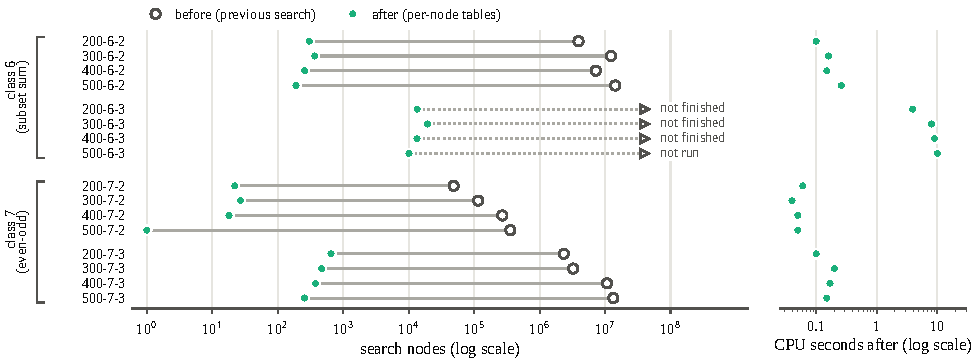
\includegraphics{figures/fig_kip_search}
\caption{Search nodes for the \NumNewKip{} knapsack interdiction instances open in the
literature, before and after the per-node tables (left, log scale), and CPU seconds after (right,
log scale). Labels: items-class-index of \code{interKP-}\emph{items}\code{-100-}\emph{class}\code{-}\emph{index}.
All are proven optimal, the slowest (\inst{\KipHardestName}, optimum \KipHardestOptimum) in
\KipHardestNodes{} nodes and \KipHardestCpu{} seconds.}\label{fig:kipsearch}
\end{figure}

\subsection{The OR Set}\label{sec:res-or}

Table~\ref{tab:or} and Figure~\ref{fig:orgaps} show the relative optimality gap $(U-L)/U$, where
$L$ and $U$ are the best lower and upper bounds from the literature and this work (the upper bound
may be an unverified published point), over the instances with both a published lower and a
published upper bound. The published points come from Lozano, Bergman and
Cire\cite{lozano2026network,lozano_dbo_repo} and Lefebvre and Schmidt.\cite{lefebvre2025dantzig}
At \NumOrInconsistent{} instances a published lower bound exceeds a published point; these are left
out of the medians and listed in Supp.\ Table~S6. For three of them, \OrConflictNames, the point
is one of Lefebvre and Schmidt's, from runs stopped at a time or solution limit, and lies below
Lozano et al.'s lower bound. With one follower knapsack the median gap falls from
\OrGapOneQuarterLit\% to \OrGapOneQuarterNow\% at budget 25\% and from \OrGapOneHalfLit\% to
\OrGapOneHalfNow\% at budget 50\%; at budget 75\% the published bounds were already tight. With
several follower knapsacks the lower bounds are the literature's, so the gaps move only through
better points: little at budget 25\%, much more at 75\%.

\begin{table}[t]
\caption{Median relative gap $(U-L)/U$ on the OR set over the instances with both a published
lower and upper bound (paired; the \NumOrInconsistent{} instances with conflicting published bounds
left out), with the literature alone and with this work added, and the instances without any
published point.}\label{tab:or}
\centering\small
\begin{tabular}{@{}l c r S[table-format=2.2] S[table-format=2.2] r r@{}}
\toprule
 & & & \multicolumn{2}{c}{Median gap (\%)} & \multicolumn{2}{c}{No published point}\\
\cmidrule(lr){4-5}\cmidrule(l){6-7}
Follower knapsacks & Budget & Paired & {Literature} & {Now} & Instances & First point here\\
\midrule
One (\code{-100}) & 25\% & \OrPairedOneQuarter & \OrGapOneQuarterLit & \OrGapOneQuarterNow & \OrNoPointOneQuarter & \OrFirstOneQuarter\\
 & 50\% & \OrPairedOneHalf & \OrGapOneHalfLit & \OrGapOneHalfNow & \OrNoPointOneHalf & \OrFirstOneHalf\\
 & 75\% & \OrPairedOneThreeQuarter & \OrGapOneThreeQuarterLit & \OrGapOneThreeQuarterNow & \OrNoPointOneThreeQuarter & \OrFirstOneThreeQuarter\\
\addlinespace
Several (\code{-0}) & 25\% & \OrPairedZeroQuarter & \OrGapZeroQuarterLit & \OrGapZeroQuarterNow & \OrNoPointZeroQuarter & \OrFirstZeroQuarter\\
 & 50\% & \OrPairedZeroHalf & \OrGapZeroHalfLit & \OrGapZeroHalfNow & \OrNoPointZeroHalf & \OrFirstZeroHalf\\
 & 75\% & \OrPairedZeroThreeQuarter & \OrGapZeroThreeQuarterLit & \OrGapZeroThreeQuarterNow & \OrNoPointZeroThreeQuarter & \OrFirstZeroThreeQuarter\\
\addlinespace
Several (\code{-50}) & 25\% & \OrPairedFiftyQuarter & \OrGapFiftyQuarterLit & \OrGapFiftyQuarterNow & \OrNoPointFiftyQuarter & \OrFirstFiftyQuarter\\
 & 50\% & \OrPairedFiftyHalf & \OrGapFiftyHalfLit & \OrGapFiftyHalfNow & \OrNoPointFiftyHalf & \OrFirstFiftyHalf\\
 & 75\% & \OrPairedFiftyThreeQuarter & \OrGapFiftyThreeQuarterLit & \OrGapFiftyThreeQuarterNow & \OrNoPointFiftyThreeQuarter & \OrFirstFiftyThreeQuarter\\
\bottomrule
\end{tabular}
\end{table}

\begin{figure}[t]
\centering
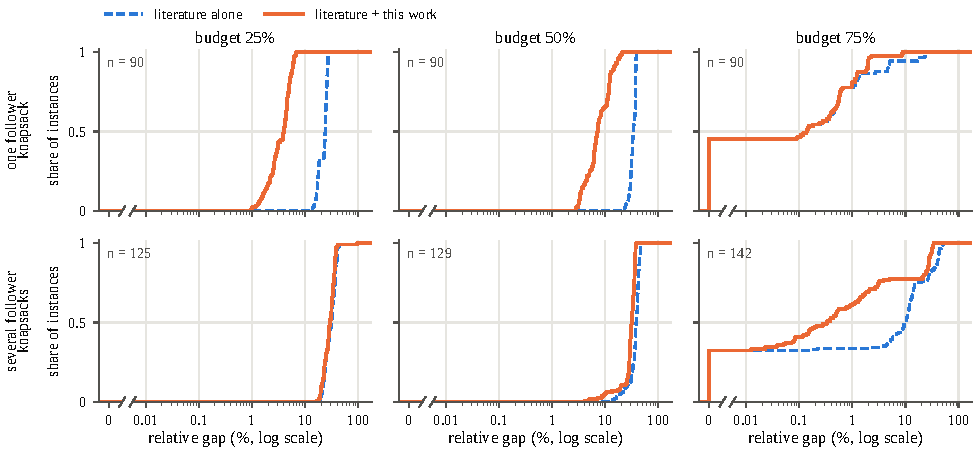
\includegraphics{figures/fig_or_gaps}
\caption{Relative optimality gap $(U-L)/U$ on the OR set over the instances with both published
bounds (the \NumOrInconsistent{} with conflicting published bounds left out), literature alone
against literature plus this work, by follower type and budget (cumulative share; $n$: instances
in the panel). Gaps of 0, closed instances, are drawn at the separate ``0'' tick; no gap is
negative.}\label{fig:orgaps}
\end{figure}

Of the \NumOr{} OR instances, \NumOrPoints{} now have a verified point: all \NumOrOneKnapsack{}
with one follower knapsack, all \NumOrSeveralHigh{} with several follower knapsacks at budget 50\%
or 75\%, and \NumOrSeveralQuarterPoints{} of the \NumOrSeveralQuarter{} at budget 25\%
(Figure~\ref{fig:orimp}). Compared with the best published point, BOBILib's included,
\NumOrBetter{} of these points are strictly better, \NumOrEqualPublished{} are equal and
\NumOrWorsePublished{} are worse; for \NumOrFirstAnywhere{} instances the point is the first
anywhere. For \NumOrPointNewToBobilib{} more it is the first in BOBILib, although Lozano et al.\
had published one. With one follower knapsack the LP bracket and the merged-row online bound give
a better lower bound than the published one for \NumOrBetterLb{} instances.

\begin{figure}[t]
\centering
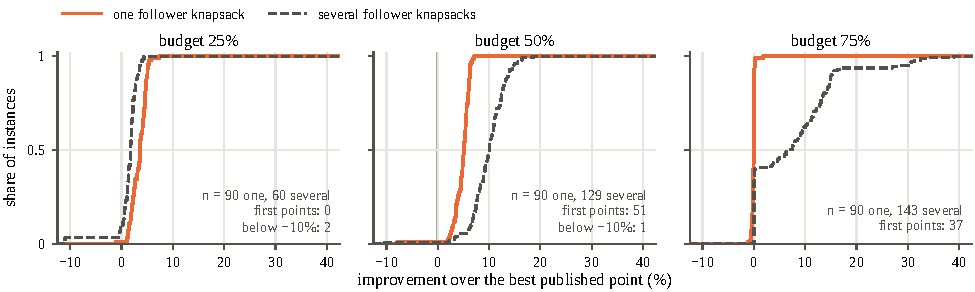
\includegraphics{figures/fig_or_improvement}
\caption{Improvement of the verified OR points over the best published point (literature or
BOBILib), by budget and follower type (cumulative share). In each panel, ``compared'' gives the
points compared with one and with several follower knapsacks, ``first points'' the instances with
no published point (not shown), and ``left of $-10\%$'' the points off the scale on the left; the
three points of instances with conflicting published bounds are left out. Of the \NumOrPoints{}
points, \NumOrBetter{} are strictly better.}\label{fig:orimp}
\end{figure}

One published optimum needs a note. For \inst{\OrClosureName} Lozano, Bergman and Cire published a
point of value \OrClosureValue{} and, in their paper's table, a lower bound of \OrClosureLitLb{}
from runs they flag as numerically inconsistent; their repository also records a branch-and-cut
bound of \OrClosureValue{}.\cite{lozano_dbo_repo} The point and the branch-and-cut bound prove the
value optimal, so the instance is counted among the published optima. The verified solution file
of this work at \OrClosureValue{} (checked also with SCIP) confirms that the bound
\OrClosureLitLb{} is wrong.

\subsection{Clique Interdiction}\label{sec:res-clique}

Of the \NumCliqueSet{} clique instances, \NumNewClique{} are optimal (Figure~\ref{fig:cliquevalues}):
\NumCliqueSevenThree{} at density 0.7 with value \CliqueOptSeven{} and all \NumCliqueNineFour{}
at density 0.9 with value \CliqueOptNine{}, where BOBILib lists \CliqueBobiMin{} to
\CliqueBobiMax{}. BOBILib's points are valid feasible points; their leader choices are just far
from optimal. The \NumCliqueOpen{} open instances, \CliqueOpenNames{}, have value
\CliqueOpenLower{} or \CliqueOpenUpper{}. Value \CliqueOpenLower{} needs a set of at most
$k=\CliqueOpenK$ edges that meets every $K_4$. The best 3-partitions found have
\CliqueOpenBestThreeA{}, \CliqueOpenBestThreeB{} and \CliqueOpenBestThreeC{} inside edges, and
searches that are not restricted to 3-partite remainders stop at the same values. A proof of value
\CliqueOpenUpper{} cannot use Brouwer's theorem: $m-k=\CliqueMantelLhsSixty$ is far below its
threshold $\CliqueBrouwerRhsSixty$, and there are $K_4$-free graphs with that many edges that are
not 3-partite (\supp{D.6}). LP bounds on the smallest such edge set stop near
\CliqueOpenLpBound{}.

\begin{figure}[t]
\centering
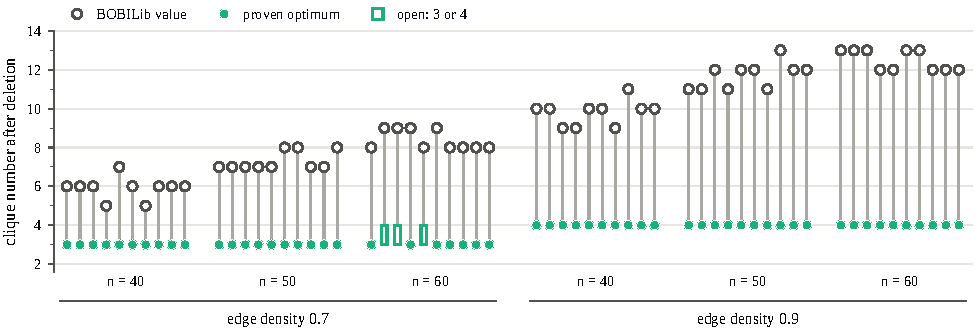
\includegraphics{figures/fig_clique_values}
\caption{The \NumCliqueSet{} clique interdiction instances: BOBILib's value (\CliqueBobiMin{} to
\CliqueBobiMax{}, open circle) against the proven optimum (\CliqueOptSeven{} at density 0.7,
\CliqueOptNine{} at density 0.9). The \NumCliqueOpen{} open instances lie between
\CliqueOpenLower{} and \CliqueOpenUpper{}.}\label{fig:cliquevalues}
\end{figure}

\subsection{Network and General Instances}\label{sec:res-general}

The network instances \inst{tree-50\_1-5-5\_006} and \inst{tree-50\_1-5-5\_010} are optimal at
\NetworkOptimum{}, BOBILib's value; \NetworkOptAttacksA{} and \NetworkOptAttacksB{} of the
\NetworkAttacks{} attacks reach it. Of BOBILib's \NetworkBobiOptimal{} optimal network values,
\NetworkRederived{} are derived again: the \NetworkTreesReproduced{} trees by the same code, the
\NetworkRndSmall{} random graphs with 25 nodes by HiGHS at every attack, and \NetworkReviewOnly{}
random graphs with 50 or 80 nodes by the brute force of the separate review.

Figure~\ref{fig:general} shows the outcome for the \NumGeneralUnsolved{} unsolved general
instances. Of the instances that BOBILib lists as open, \NumNoFeasible{} have no bilevel feasible
point: \NumRayExact{} certificates pass the exact rational check, and for the other \NumRayFloat{}
(\inst{supportcase42\_0\_100} and \inst{supportcase42\_50\_50}) small rounding residuals remain,
so they rest on floating point. Without coupling rows, \code{bobi general} was run on
\NumGeneralCandidates{} open instances. \NumGeneralCandRays{} of them have no bilevel feasible
point, and of the other \NumGeneralCandWithPoint{} it gives verified points for
\NumGeneralFiles{}. For \NumGeneralNoCplPublished{} of these a point had been published elsewhere,
better than ours for \NumGeneralNoCplPublishedBetter{} (Supp.\ Table~S12); for the others it is the
first point known. With coupling rows, \code{bobi coupled} was run on \NumCoupledAttempted{} of
\NumCoupledCandidates{} candidates and found \NumCoupledFiles{} verified points:
\NumCoupledByHpr{} at the HPR's own leader values, \NumCoupledByPenalty{} from the penalized HPR
and \NumCoupledByFollow{} from best-response dynamics. In \NumCoupledTolerance{} of these files the
follower's value lies about $10^{-7}$ relative above its optimum, within BOBILib's
test~\eqref{eq:tol}, and the leader uses that slack. The files for \inst{pg\_50\_50} and
\inst{neos-2978193-inde\_50\_50} are feasible only within that tolerance, although both instances
do have exactly bilevel feasible points (\supp{E.4}).

\begin{figure}[tb]
\centering
\begin{minipage}[b]{3.15in}
\centering
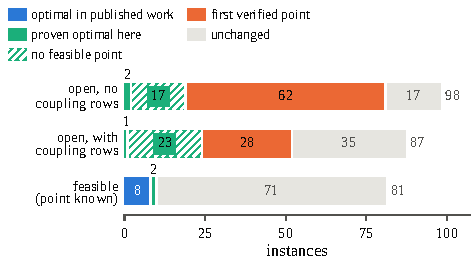
\includegraphics{figures/fig_general_outcomes}
\caption{Outcomes for the \NumGeneralUnsolved{} general instances BOBILib lists as feasible or
open, by BOBILib status and, for the open ones, by whether leader rows contain follower
variables (coupling rows).}\label{fig:general}
\end{minipage}\hfill
\begin{minipage}[b]{3.33in}
\centering\small\setlength{\tabcolsep}{3pt}
\captionof{table}{Instances whose HPR is exactly the MIPLIB model they were built from, with a
verified point at its published optimum. BOBILib: status before this work; point from: BOBILib's
solution file or the method of this work. MIPLIB's optimum
of noswot, \NoswotMiplibOptimum{}, rounds up because its objective takes integer values
only.}\label{tab:hpr}
\begin{tabular}{@{}l l r l@{}}
\toprule
Instance & BOBILib & Optimum & Point from\\
\midrule
\HprTableRows
\bottomrule
\end{tabular}
\end{minipage}
\end{figure}

Table~\ref{tab:hpr} lists the \NumHprOptimal{} instances that are optimal at the MIPLIB bound.
Of these, \inst{pigeon-10\_0\_100}, \inst{pigeon-10\_50\_50} and \inst{timtab1\_0\_100} were open,
with no point known. For \inst{noswot\_0\_100} and \inst{noswot\_50\_50} BOBILib's own points
already had the optimal value; the proof is new. The generalized interdiction instances that
remain unchanged (\NumGeneralizedUnchanged{} of them) have many linking variables: enumerating
their binary linking choices, which reproduces a published optimum on a smaller instance of the
set, is too slow for them.

% ======================================================================================
\section{Discussion}\label{sec:discussion}

The new results come from structure, certificates and published bounds that a general-purpose
MIBLP solver does not use. A general branch and bound over the \CliqueMSixtyNine{} edge variables
of a 60-vertex clique instance at density 0.9 is unlikely to show quickly that every deletion of
\CliqueKSixtyNine{} edges leaves a $K_4$, while Brouwer's theorem and \NumCliquePartCases{} small
cases do; and an instance without a bilevel feasible point needs one direction as a certificate,
while a solver that searches for a point can only report a time limit.

\subsection{Recommendations for Benchmark Libraries}

Benchmark statuses are most useful when they are current and when each comes with its evidence.
From this work I suggest:
\begin{itemize}
\item record the provenance of every status (a solver run with its limits, a published proof, or
a certificate), and import published per-instance results, so that an instance solved elsewhere
is not listed as unsolved;
\item screen new instances for followers that are infeasible or unbounded for every leader
choice, and accept certificates of bilevel infeasibility, such as the recession directions here,
as evidence for an infeasible status;
\item state the tolerances behind every status, and prefer exactly optimal follower responses.
In BOBILib's solution file for the generalized interdiction instance
\inst{general20-30-20-20-20-2} the follower's value is \GenTolPhiSol{}, while the follower's
optimum at the same leader choice is \GenTolPhiOpt{}: \GenTolDiff{} units, or \GenTolRel{}
relative, above it. Test~\eqref{eq:tol} accepts this because the follower's values are large, and
the rows, violated by up to \GenTolViolation{}, pass the $10^{-4}$ tolerance of the MIPLIB
checker inside BOBILib's checker (\supp{A.2}). \code{bobi verify} rejects the file: it does not
meet the rows within $10^{-6}$, and its stated objective \GenTolObjFile{} differs from the
\GenTolObjComputed{} of its point (\supp{E.5}). This work is not free of the issue either:
\NumCoupledTolerance{} of its coupled files use the follower slack of Table~\ref{tab:tol}, and
with an exactly optimal follower their leader values are slightly worse (listed in the data
package);
\item distribute solution files and certificates in standard formats, with a status file in the
MIPLIB \code{.solu} format, as the data package of this paper does.
\end{itemize}

\subsection{Limitations and Threats to Validity}\label{sec:limits}

\textbf{Running times.} All times come from a shared four-core machine that was often
oversubscribed; they show orders of magnitude, not careful benchmarks.

\textbf{Floating point and tolerances.} The points are feasible within $10^{-6}$ and
follower-optimal within BOBILib's relative tolerance, not exactly, and \NumCoupledTolerance{}
coupled points use that slack (Section~\ref{sec:res-general}). Of the \NumNoFeasible{} recession
certificates, \NumRayFloat{} are checked only in floating point; the status file marks them. The
MIPLIB optima behind the \NumHprOptimal{} bound-based optima are published floating-point values;
\inst{timtab1\_0\_100}, for example, is optimal at \TimtabOptimum{}, the value MIPLIB prints as
\TimtabOptimumRounded{}. The LP bracket and the merged-row bound are evaluated in double precision,
and the window rule of the subset-sum search uses a floating-point fractional bound; the
\NumNewKip{} subset-sum proofs are confirmed by the integer-only provers, which do not use that
rule.

\textbf{Trusted solvers.} Follower optimality for followers with several rows and for general
instances, the \NumCliquePartCases{} part-size verdicts and the dual bounds of the OR bracket come
from MILP and constraint programming solvers. The part-size verdicts were reproduced by several
methods, two of them solver-free, but a bug that all methods share would go unnoticed. Certificates
in a checkable proof format, such as VIPR for MILP verdicts\cite{cheung2017verifying} from an
exact rational solver\cite{eifler2023computational} or pseudo-Boolean proof logs checked by
VeriPB,\cite{bogaerts2023certified} would remove this trust; they were not produced here.

\textbf{Scope of the Lean proofs.} Lean covers the main pruning lemmas of the KIP search and the
Mantel and partition lemmas for clique interdiction. It does not cover the reduction to the count
formulation, the cheaper rules of Supp.\ Thm~B.23, Brouwer's theorem, the LP bracket, the network
DP, the recession directions, or the search code itself (Table~\ref{tab:lean}).

\textbf{Results taken from the literature.} The \NumLitOptimal{} published optima, the work of
their authors, and the published lower bounds of the OR instances with several follower
knapsacks are used as reported; for \NumLitNoFile{} of the optima not even a point is verified
here. ``First point anywhere'' means that none of the published sources
compiled here (Supp.\ Sec.~H) has a point; for \NumGeneralPublishedPoint{} of the general
instances given a point by \code{bobi general} or \code{bobi coupled} a published point exists
(for \NumGeneralPublishedLS{} of them only in Lefebvre and Schmidt's run files), and these are not
counted as first points. Other sources may hold points that this reconciliation missed.

\textbf{Common-mode errors.} The solvers, the verifier and the separate review sessions were all
written with the same AI coding agent directed by the same author. Separate sessions with their own
code and instance readers reduce, but do not remove, the risk of a shared misreading of the file
format or a shared conceptual slip. The Lean proofs, the exact rational checks and the
brute-force comparisons are the checks least exposed to it.

\textbf{Instance reading.} Every argument depends on reading the instance files correctly. Each
family's model was checked row by row against its expected pattern, and the key results were
derived again with separately written readers.

\subsection{What Stays Hard}

For the \NumCliqueOpen{} open clique instances, value \CliqueOpenLower{} needs a set of at most
$k$ edges that meets every $K_4$, which no search has found, and value \CliqueOpenUpper{} needs a
lower bound on the size of such a set well above the LP bounds. For random graphs the
largest $K_4$-free subgraphs are 3-partite,\cite{babai1990extremal,brightwell2012extremal} which
would point to value \CliqueOpenUpper{}, but these results are asymptotic and give no bound for a
given graph with 60 vertices. The OR instances with several follower knapsacks at budget 25\% still
have no certified point in \NumOrSeveralQuarterNoPoint{} cases: \NumOrQuarterNoPointNoPub{} have no
point anywhere, and \NumOrQuarterNoPointPub{} have only a published, unverified point. Their median
gaps stay near \OrGapZeroQuarterNow\% and \OrGapFiftyQuarterNow\%; they need a lower bound that uses
the structure of several knapsacks, which the one-row bracket does not. Generalized interdiction with
many linking variables needs a pruned enumeration of the linking choices, and
\NumGeneralUnchanged{} general instances (\NumGeneralUnchangedMiplib{} of them MIPLIB-derived)
remain without a point or without a proof. The results of this work will be submitted to BOBILib's
maintainers, who update the statuses from submitted solutions.

% ======================================================================================
\section{Conclusions}\label{sec:conclusions}

I asked which of BOBILib's \NumUnsolved{} feasible or open instances can be settled. The key
findings are:
\begin{itemize}
\item Published work had already solved \NumLitOptimal{} of them; reconciling BOBILib's statuses,
which predate some of these results, with the literature settles more instances than any single
method.
\item Structure-specific methods settle \NumSettledHere{} more: a robust subset-sum search proves
all \NumNewKip{} remaining knapsack interdiction instances optimal; extremal graph theory, with
partition certificates and \NumCliquePartCases{} cases decided by exact solvers, settles
\NumNewClique{} of \NumCliqueSet{} clique interdiction instances; recession directions show that
\NumNoFeasible{} instances have no bilevel feasible point (\NumRayExact{} checked exactly);
published MIPLIB optima prove \NumNewHpr{} more optimal; and exhaustive enumeration with an exact
tree dynamic program settles the \NumNewNetwork{} network interdiction instances.
\item In all, \NumSettled{} instances (\PctSettled\%) are settled. \NumFirstPoint{} instances get a
verified point where BOBILib lists none, \NumFirstAnywhere{} of them the first point anywhere, and
\NumOrBetter{} OR instances get a point better than any published one.
\item The claims can be checked: solution files in BOBILib's format pass a separate verifier
modeled on BOBILib's checker, the certificates are published, and the main pruning lemmas of the
new search are proved in Lean.
\end{itemize}

% ======================================================================================
\section*{DATA AVAILABILITY}

The data package is the folder \code{results/} of the repository \repourl{} (archived with
DOI \datadoi). It contains \code{instances.csv}, one row per BOBILib instance with BOBILib's
status and value, the new status, the best verified value and proven bound, the source, the
method and the certificate; \code{bobilib\_update.solu}, the status changes in MIPLIB's
\code{.solu} format (\NumSoluOpt{} \code{=opt=}, \NumSoluInf{} \code{=inf=}, \NumSoluBest{}
\code{=best=} and \NumSoluBestDual{} \code{=bestdual=} lines; its header marks the \NumRayFloat{}
\code{=inf=} lines that rest on floating-point certificates); the solution files in BOBILib's
format; the certificates (recession directions, clique partitions with the solver logs of the
part-size proofs, subset-sum proof records, enumeration summaries, OR bounds); and
\code{SHA256SUMS}, the checksums of every file. The code is in the same repository: the Rust crate
\code{bobi} (the solvers and the verifier), the scripts of the separate checks, and the Lean
project with the proofs. The supplementary document (\code{paper/appendix/} in the repository)
holds the proofs, the verification protocol, the map of the Lean theorems and the per-instance
tables.

\section*{ACKNOWLEDGEMENTS}

The software development, the computational experiments, the separate review sessions and the
drafting of this paper were carried out with substantial assistance from an artificial
intelligence (AI) coding agent (Claude Code, Anthropic) directed by the author. The reviews
described in Section~\ref{sec:lean} were separate sessions of the same agent that wrote their own
code. All results were checked by the verification described in Sections~\ref{sec:verify}
and~\ref{sec:lean}. I thank the maintainers of BOBILib, Johannes Th\"urauf, Thomas Kleinert, Ivana
Ljubi\'c, Ted Ralphs and Martin Schmidt, for the library, its solution files and its checker, and
the authors who published their per-instance data and code, in particular Noah Weninger and
Ricardo Fukasawa; Matteo Fischetti, Ivana Ljubi\'c, Michele Monaci and Markus Sinnl; Leonardo
Lozano, David Bergman and Andre A.\ Cire; and Henri Lefebvre and Martin Schmidt.

\bibliographystyle{spiebib-doi}
\bibliography{refs}

\end{document}
